% mnras_template.tex 
%
% LaTeX template for creating an MNRAS paper
%
% v3.0 released 14 May 2015
% (version numbers match those of mnras.cls)
%
% Copyright (C) Royal Astronomical Society 2015
% Authors:
% Keith T. Smith (Royal Astronomical Society)

% Change log
%
% v3.0 May 2015
%    Renamed to match the new package name
%    Version number matches mnras.cls
%    A few minor tweaks to wording
% v1.0 September 2013
%    Beta testing only - never publicly released
%    First version: a simple (ish) template for creating an MNRAS paper

%%%%%%%%%%%%%%%%%%%%%%%%%%%%%%%%%%%%%%%%%%%%%%%%%%
% Basic setup. Most papers should leave these options alone.
\documentclass[fleqn,usenatbib]{mnras}

% MNRAS is set in Times font. If you don't have this installed (most LaTeX
% installations will be fine) or prefer the old Computer Modern fonts, comment
% out the following line
\usepackage{newtxtext,newtxmath}
% Depending on your LaTeX fonts installation, you might get better results with one of these:
%\usepackage{mathptmx}
%\usepackage{txfonts}

% Use vector fonts, so it zooms properly in on-screen viewing software
% Don't change these lines unless you know what you are doing
\usepackage[T1]{fontenc}
\usepackage{float}
\usepackage{enumerate}

% Allow "Thomas van Noord" and "Simon de Laguarde" and alike to be sorted by "N" and "L" etc. in the bibliography.
% Write the name in the bibliography as "\VAN{Noord}{Van}{van} Noord, Thomas"
\DeclareRobustCommand{\VAN}[3]{#2}
\let\VANthebibliography\thebibliography
\def\thebibliography{\DeclareRobustCommand{\VAN}[3]{##3}\VANthebibliography}


%%%%% AUTHORS - PLACE YOUR OWN PACKAGES HERE %%%%%

% Only include extra packages if you really need them. Common packages are:
\usepackage{graphicx}	% Including figure files
\usepackage{amsmath}	% Advanced maths commands
% \usepackage{amssymb}	% Extra maths symbols
\usepackage{subfigure}
\usepackage{siunitx}
\usepackage{array}
%%%%%%%%%%%%%%%%%%%%%%%%%%%%%%%%%%%%%%%%%%%%%%%%%%

%%%%% AUTHORS - PLACE YOUR OWN COMMANDS HERE %%%%%

% Please keep new commands to a minimum, and use \newcommand not \def to avoid
% overwriting existing commands. Example:
%\newcommand{\pcm}{\,cm$^{-2}$}	% per cm-squared

%%%%%%%%%%%%%%%%%%%%%%%%%%%%%%%%%%%%%%%%%%%%%%%%%%

%%%%%%%%%%%%%%%%%%% TITLE PAGE %%%%%%%%%%%%%%%%%%%

% Title of the paper, and the short title which is used in the headers.
% Keep the title short and informative.
\title[Short title, max. 45 characters]{Measuring the evolution of early-type galaxies in GAMA using observationally robust  quantities}

% The list of authors, and the short list which is used in the headers.
% If you need two or more lines of authors, add an extra line using \newauthor
\author[Rongfu Liu et al.]{
Rongfu Liu$^{1}$, 
Alessandro Sonnenfeld$^{1}$\\
$^{1}$Department of Astronomy, School of Physics and Astronomy, Shanghai Jiao Tong University, Shanghai, China
% List of institutions
}

% These dates will be filled out by the publisher
\date{Accepted XXX. Received YYY; in original form ZZZ}

% Enter the current year, for the copyright statements etc.
\pubyear{2023}

% Don't change these lines
\begin{document}
\label{firstpage}
\pagerange{\pageref{firstpage}--\pageref{lastpage}}
\maketitle

% Abstract of the paper
\begin{abstract}
Quiescent galaxies today is believed to have experienced more dramatic growth in their evolution history, comparing their star-forming counterpart. Traditionally, most of the method used to investigate the evolution of these object involved the total light of one galaxy, which we believed to be not well-defined and is likely to suffer from extrapolation problem. To eliminate such potential bias, we use a different parameterization, namely $M_{*,10}$ and $\Gamma_{*,10}$ which is the mass and the mass-weighted density slope enclosed in circularised aperture $10$kpc, respectively. We first explore the $\Gamma_{*,10} - M_{*,10}$ relation for a sample of quiescent galaxies from GAMA survey combining with the KiDs image, and find a steeper slope for galaxies with lower redshift. We then analyzed a collection of binary-merger simulations which contains mergers with different merger mass ratio. From the simualtion result we could directly observe that mergers would always induce a decrease in $\Gamma_{*,10}$ , but might induce a counter-intuitive increase in $M_{*,10}$ for larger galaxies and smaller merger mass ratio. We then built a toy model to predict the evolution in $\Gamma_*{*,10} - M_{*,10}$ relation, and found that for every merger mass ratio, the slope would always increase and the normalization would always decrease, while the change would become more intensive for smaller merger mass ratio. Comparing with the observation result, we believe galaxies do grow during redshift range $0.15 \leq z \leq 0.40$, and the growth should be driven by mergers with merger mass ratio lower than 1:5.
% analyses a collection of binary-merger simulations and find that the growth in $M_{*,10}$ and $\Gamma_{*,10}$ are different in different merger scenarios and different galaxies size. We then select a $M_{*,10}$ complete sample of galaxies in GAMA survey and use KiDs r-band image to provide structural parameters. We measured $M_{*,10}$ and $\Gamma_{*,10}$ for these galaxies, and compare the evolutionary trend with simulation results. We find that for galaxies with $M_{*,10} \geq 10^{10.9} M_{\odot}$ and redshift $0.15 \leq z \leq 0.40$, no significant evidence shows they experienced a growth due to merger of any kinds.  
\end{abstract}

% Select between one and six entries from the list of approved keywords.
% Don't make up new ones.
\begin{keywords}
keyword1 -- keyword2 -- keyword3
\end{keywords}

%%%%%%%%%%%%%%%%%%%%%%%%%%%%%%%%%%%%%%%%%%%%%%%%%%

%%%%%%%%%%%%%%%%% BODY OF PAPER %%%%%%%%%%%%%%%%%%

\section{Introduction}
\label{sec:intro}
% \cite{van_dokkum_1996}
\par Early type galaxies (ETGs), which are typically elliptical in shape, are believed to have complete most of their star-forming activities before the epoch of $z \approx 2$ and are passively evolved afterwards.Besides the focus on what mechanism that shut down the star formation, the passive evolving process of these galaxies is also a highly debated subjects in the field of galaxy evolution.Obtaining a better understanding on this process could help us better understand the hierarchical structure formation theory, which is a fundamental theory in $\Lambda$CDM cosmology.
\par  Over the past few decades, observations have suggested that quenched ETGs are much more compact than their counterpart at $z \approx 0$ \citep{daddiPassivelyEvolvingEarlyType2005, toft2007, trujillo2006, trujillo2007, vandokkum2008}. As a consequence, the passive evolution process of the quiescent, ultra-compact objects experienced are believed to have induced a dramatic growth in size, in particular, by about a factor of 3 between $z = 2$ and $z = 0$ \citep{damjanov2019, fan_dramatic_2008, hamadouche2022, vanderwel3DHSTCANDELSEvolution2014, van_dokkum_growth_2010}.
% have a more significant growth in size comparing to their star-forming counterpart.
% Currently, the most popular formation scenario of ETGs consists of two phases. At early time ($z > 2$), proto-ellipticals are formed in an intense star-forming activities with strong gas dissipation process which drive these galaxies to be extremely compact. Most of the stellar mass of such systems are gained through this first phase of formation. While in the second phase, it is well agreed that the growth was dominated by minor mergers, resulting in a "puffing-up" in size and a moderate growth in stellar mass.
Given that the star formation rate of these ETGs are relatively low, \cite{van_dokkum_growth_2010} suggested that the these galaxies should have experienced a built-up process of their outer envelope since $z \approx 1.5$ via some form of merging and accretion.
% Numerous works in literature have discovered that the dissipationless dry mergers could be one possible major mechanism that attribute to that rapid size growth. 
% In fact, different merger ratios are believed to be able to leave different impacts on various properties of galaxies.
 Numerous works in literature that based on both observations and hydrodynamic simulations have suggested that the dissipationless dry mergers might be the major growth mechanism, as it could explain the evolution in size, density profile, central densities and  orbital structures of these quiescent galaxies 
\citep{naab_minor_2009, van_dokkum_2010_hubble, oser_cosmological_2011, newman2012, hilz_how_2013, dekel_wet_2014, deugenio2023}. In particular, minor mergers, which means the mass ratio between the accreted galaxy and the progenitor galaxy is relatively small, are believed to have dominated the merger event that one galaxy might experience, especially for mergers with mass ratio around 1:10 \citep{newman2012, Belli_2015}. Taking the advantage of the depth and resolution of JWST Advanced Deep Extragalatic Survey \citep{Gardner_JWST,Eisenstein_JADES}, we are enabled to detect very low mass ratio ($ \leq 1:100$)mergers.The result also suggest that mergers with ratio close to 1:10 are likely to drive the size growth while lower mass ratio mergers might dominate the color gradients evolution \citep{Suess2023}. 
\par However, although minor merger scenario has made a great success in explaining the evolution of ETGs, there's still some issues that has not been solved. For instance, at redshift $z \geq 1$, minor mergers alone seems insufficient. Both observations and prediction seems to suggested a more rapid growth rate due to the accretion with satellite galaxies, comparing to the predicted value we made with the assumption that all the accreted mass are from minor mergers \citep{hopkins_discriminating_2010,nipoti2009}.The evolution in the density slope of galaxies in this minor merger scenario might also not be consistent with observations \citep{sonnenfeld2014}. While at intermediate redshift, a mass-dependent growth rate is suggested, but the result seems less conclusive. \cite{vanderwel3DHSTCANDELSEvolution2014,KiDs_Roy} found out that the massive ETGs ($M_* \geq 10^{11} M_\odot$)are likely to grows most rapid in size, comparing to less massive counterparts. While \cite{damjanov2019} suggest a contrast trend, she found the size growth of massive quiescent galaxies are significantly slower than that of less massive ones. She suggested that mechanism that drives the size growth may have altered in this intermediate redshift range, thus detailed observation should pay more attention to that epoch. In fact, taking the result from \cite{Bundy2017} into consideration, which do not suggest a significant growth in number density of massive ETGs during $0.3 < z < 0.65$, we cannot conclude for sure if and how that quiescent galaxies grow at this intermediate redshift range.
\par To further investigate this issue, we also need to deal with the systematics carefully.The existence of systematics would limit our ability to measure the growth of ETGs precisely.
 Among various systematics, the progenitor bias is one that commonly addressed in literature. The population of quiescent galaxies are not static, star-forming galaxies could be quenched and join the quiescent population continuously.If these "fresh bloods" are relatively larger,the change in demography could thus mimic the evolution in average size that minor merger process may induce\citep{van_dokkum_1996,carolloNEWLYQUENCHEDGALAXIES2013, fagioliMinorMergersProgenitor2016, vandokkumMorphologicalEvolutionAges2001}.
% A detailed theoretical model are still in absence to explained what 
In fact, our understanding about the growth of quiescent galaxies could still be improved, a detailed theoretical model that could take some additional minor mechanisms (e.g. major mergers) and possible systematic (e.g. progenitor bias) into account is still in absence.
\par Besides, another possible systematic might be ignored in the literature.The problem arise from the finite photometric depth of observations.It is hard to measure the total light directly \citep{tal_2011_faint} as the information where the surface brightness of galaxies drops below the observation limit remains unknown. To obtain a accurate measurement of the total light, a precise sky-subtraction is demanded, while it is easy to bring additional systematic. In literature, we use various models to fit the surface brightness distribution of galaxies . The faint outskirt of galaxies could not provide reliable constrains during the fitting process, thus the model could not be able to provide reliable descriptions for surface brightness there . These unreliable data will be accounted in the total light measurement and will take up an ineligible fraction\citep{Alessandro20}.However, the traditional definition of galaxy size and mass derived from the best-fit model are both associated with the total light, therefore we believe they are not robust qualities. 
% Both half-light radius and total stellar mass that derived from the best-fit model are associated with total light , and thus we believe that the traditional definition of galaxy size and mass is not robust. 
\par One of the main goal of this work is to eliminate the possible bias that introduced by the data measured in the unreliable outer region of galaxies. 
% In order to eliminate the influence of unreliable data in the outer region of galaxies, 
In particular, we switch our focus from the entire galaxy to a fixed, relatively small aperture following the method proposed in \cite{Alessandro20}. In this work, we choose 10kpc as that aperture,in consideration that it is large enough to enclose sufficient amount of stellar mass while will not be too large to suffer from the extrapolation problem. We use $M_{*,10}$ to denote the mass enclosed inside 10kpc and $\Gamma_{*,10}$ to represent to mass-weighted projected surface density slope.The latter is defined as
\begin{equation}
    \label{eq:gammastar10}
    \Gamma_{*,10} = \frac{2\pi \int_0^{10} R \frac{dlog\Sigma_*}{dlogR}\Sigma_*(R)dR}{2\pi \int_0^{10}R\Sigma_*(R)dR} = 2 - \frac{2\pi \times 10^2 \times \Sigma_*(10)}{M_{*,10}}
\end{equation} 
We replace the traditional definition of galaxy size(effective radius $R_e$) and stellar mass($M_*$) with these two quantities, thus the relation between $M_{*,10}$ and $\Gamma_{*,10}$ could provide a new insight into the traditional scaling relation. With the help of these new robust quantities, we hope to answer the following questions:
\begin{enumerate}[1.]
    \item Whether quiescent galaxies grow in a given redshift range?
    \item If galaxies do growth, what could be the possible mechanisms that drive the growth?
\end{enumerate}
% \par In context of merger, the growth in size of one single galaxies can be approximated by Virial Theorem, assuming a isothermal density profile( \cite{naab_minor_2009}).
\par Therefore, it's necessary to understand the impact of various growth mechanism, in particular, mergers with diferent merger ratio. Assuming a isothermal density profile for elliptical galaxy, the growth in total stellar mass and effective radius due to mergers can be approximated by some simple formulas using virial theorem\citep{naab_minor_2009}.
%  we can obtain a strict relation between $\Delta M_*$ and $\Delta R_e$ depending on different merger scenarios
 . However, switching to $M_{*,10}$ and $\Gamma_{*,10}$ space, it's hard to derive a relation in $\Delta M_{*,10}$ and $\Delta \Gamma_{*,10}$ analytically as a fixed aperture size 10kpc is involved. Nevertheless, N-body simulations can be helpful. We utilize the simulation result from \cite{nipoti2009} which contains a number of binary mergers with different mass ratio. We measure the $M_{*,10}$ and $\Gamma_{*,10}$ of both progenitor and merger remnant and calculate the growth in these two quantities. In addition to finding that different merger ratio behaves differently, we also discovered that the scale of galaxy also make diferences. 
\par Having find how the $M_{*,10}$ and $\Gamma_{*,10}$ under different growth scenarios, we then compared them with the evolution of these two quantities in reality. We select ETGs from GAMA DR4 main survey (Galaxy and Mass Assembly, \cite{GAMAmain};\cite{bellstedt_galaxy_2020} ; \cite{GAMA1}; \cite{GAMA2}) and obtained precise spectroscopic redshift and other quantities that related to spectrum measurement, e.g. stellar mass. In addition, 
% we use the 2DPHOT structural parameter catalogue from KiDs DR4 
the structural parameter are measured from KiDs photometry (Kile Degree survey , \cite{kuijken_fourth_2019}, \cite{KiDs_Roy}, \cite{Amaro_rejection_2021}) using GalNet (\cite{GaLNet2022}). Based on these observation datas,  we then calculated their $M_{*,10} $ and $\Gamma_{*,10}$ and further analyse the , $M_{*,10} - \Gamma_{*,10}$ relation and their evolution from $z = 0.6$ to present. 
% * focus inside 10kpc
% \par By focusing inside $10kpc$, we are automatically able to know if and how the stellar mass of inner region grow. In the context of two-phase formation scenario of ETGs, during the second evolution phase, the total stellar mass will grow insignificantly, and is confirmed by observations recently (\cite{Bundy2017}) . In contrast, due to the undetermined mechanism that drive galaxy to extend, we are still not clear the behaviour of inner region through the second phase. In literature, \cite{van_dokkum_growth_2010} stacked the images of numerous galaxies and found the mass show no signal to grow in inner 5 kpc  of ETGs. Recently , take the advantage of the development of Integral Field Spectroscopy(IFS), several studies have been trying to recover the evolution histories using local, spatially resolved galaxies (cite). 

% Although our resolution is not comparable to MANGAs, our sample choice can extend to higher redshift with larger sample amount. While in comparison with \cite{van_dokkum_growth_2010}, we have better images, thus don't need to stack all the images. 
% \par Using $M_{*,10}$ along, we are able to study the evolution of inner region of galaxies.  Combining with $\Gamma_{*,10}$, we have a robust set of parameters to describe the mass density profile of galaxies. $\Gamma_{*,10} $ is, by definition, the average slope of the surface density profile inside 10 $kpc$, thus encode the information about how compact one galaxy is. Actually, the combination of $M_{*,10}$ and $\Gamma_{*,10}$ can provide a precise description of surface density slope in inner $10  kpc $ better than 20\% \cite{Alessandro20}. We believe it is reasonable to measure the growth in size of ETGs using this parameterization.  
% using this set of parameters, we are able to measure the evolution in density profile of ETGs and might indicate how the size of galaxies grow.   
% \par In this work, we select ETGs from GAMA DR4 main survey (Galaxy and Mass Assembly, \cite{GAMAmain};\cite{bellstedt_galaxy_2020} ; \cite{GAMA1}; \cite{GAMA2}) and obtained most of the qutities we want, such as total stellar mass, redshift etc.. In addition, we use the 2DPHOT structural parameter catalogue from KiDs DR4 ( Kile Degree survey , \cite{kuijken_fourth_2019}, \cite{KiDs_Roy}, \cite{Amaro_rejection_2021}) to give most of ETGs reasonable sersic parameters in complement. For the rest galaxies, we use GALFIT (\cite{Peng_galfit_2002}, \cite{Peng_galfit_2010}) to operate a single sersic fitting to obtain their sersic parameters. Then we calculate their $M_{*,10} $ and $\Gamma_{*,10}$ and further analyse the $M_{*,10} $ funtion, $M_{*,10} - \Gamma_{*,10}$ funtion and their evolution from $z = 0.6$ to present. 
\par The structure of this paper is as follows. We present the selection of our observational sample and the observed $\Gamma_{*,10} - M_{*,10}$ relation in Sect.\ref{sec:2}. In Sect.\ref{sec:3}, we present the details of the simulation and the toy model that we built upon the simulation, as well as the comparison between observations. Then we discussed the result in Sect.\ref{sec:4} and give a brief conclusion in Sect.\ref{sec:5}.
\par In this paper, we assume a flat $\Lambda$CDM cosmology with $\Omega_M = 0.3$ and $H_0 = 70 km ~s^{-1}~Mpc^{-1}$. Magnitude are in AB units and stellar mass are in solar units.
% In fact, $\Gamma_{*,10}$ tells us how compact one galaxy are, thus could be a reasonable indicator of the galaxy size instead of the half-light radius $R_e$.Therefore, we can use a new set of parameter $M_{*,10}, \Gamma_{*,10}$ to investigate the evolution in mass and size of ETGs.Free from the extrapolation problem, our method might be able to provide a more robust measurement of the evolution in size of ETGs. 
% That is so called extrapolation problem.
% As is expected by existing theory, the mass and size of quiescent galaxies should evolve with time, and is confirmed by the observation result at the epoch of $z > 1$(some relating papers listed here).However, approaching a closer epoch ($z < 1$), the result becomes less conclusive. Various studies has focused on the evolution of the stellar mass function\citep{Bundy2017},the mass-velocity dispersion relation \citep{2020MNRAS.498.1101C} and the mass-size relation \citep{2019ApJ...872...91D}(to be refine). 
% \par These discrepancy may come from the measurement of stellar mass and the half-light radius. Traditionally, we fit the surface brightness of galaxies with some existing model(such as Sersic model) to infer its half-light radius and total stellar mass. However, this process might be biased by extrapolation problem \cite{Alessandro20} . In the outer region of galaxy, the brightness may drop below the background noise and thus introduce profound errors. To solve this problem, we adopt the method Alessandro suggested in his paper. Instead of investigating the whole galaxy, we may focus on a fixed, relatively small aperture and investigate some properties inside. In this paper, we'll choose 10kpc as the fixed aperture,which will be large enough to enclose sufficient amount of stellar mass while will not be too large to suffer from the extrapolation problem. We use $M_{*,10}$ to denote the mass enclosed inside 10kpc and $\Gamma_{*,10}$ to represent to mass-weighted projected surface brightness slope. In fact, $\Gamma_{*,10}$ tells us how compact one galaxy are, thus could be a reasonable indicator of the galaxy size instead of the half-light radius $R_e$.Therefore, we can use a new set of parameter $M_{*,10}, \Gamma_{*,10}$ to investigate the evolution in mass and size of ETGs.Free from the extrapolation problem, our method might be able to provide a more robust measurement of the evolution in size of ETGs. 
% \par In addition, these set of parameter automatically enable us to investigate whrere and how does the growth take place. \cite{Dokkum2010} invetigated this issue and found that the stellar mass inside 5kpc won't grow with time. The method he used is stacking the images of various galaxies, which is sensitive to sky subtraction and need to make some assumptions to galaxies, such as "all galaxies are identical". Up to now, we have better observations of ETGs, and it's not necessary to stack up the images. Therefore, we don't need the assumptions mentioned above and a free from the sensitivity of the sky subtraction, and we might be able to provide a more precise result about the grow in the region of one galaxy.   
% \par In this work, we choose the ETG sample from Galaxy And Mass Assembly survey (GAMA \cite{GAMAmain}; \cite{GAMA1}; \cite{GAMA2}) and use photometric data from Kilo-Degree survey(KiDs \cite{KiDs_Roy}). We measured the $M_{*,10}, \Gamma_{*,10}$ using the Sersic parameter provided by KiDs catalogue and plot the $M_{*,10}$ function at different redshift to investigate the mass growth in the inner region of ETGs. We further studied the $M_{*,10}-\Gamma_{*,10}$ relation and it's redshift-dependent evolution.We find blablabla ......
% \par The structure of this paper is as follows. In Sect.2, We described the spectroscopic and the photometric data from GAMA survey and KiDs survey respectively, and the method we use to ensure the completeness of sample. We present the result of growth of $M_{*,10}$ and $M_{*,10}-\Gamma_{*,10}$ relation in Sect.3  and discuss the result in Sect.4. Finally, We give a brief conclusion in Sect.6   
% \section{Data}

\section{Observation}
\label{sec:2}
\subsection{Data set}
\subsubsection{Sample selection}
\par Our goal of this work is to focus on the evolution of quiescent galaxies at intermediate redshift range and attempting to elliminate a possible systematic from the extrapolation problem by focusing on a fixed aperture size $10kpc$.We expect to select a sample that consist of quiescent galaxies with spectroscopic data, hence obtain reliable measurement of redshift, stellar mass,aperture size and could distinguish them from star-forming ones. In addition, as our requirement of focusing the inner region, we need to obtain the structural parameters of galaxies in order to calculate $M_{*,10}$ and $\Gamma_{*,10}$.
\par Therefore, we choose to select galaxies based on GAMA DR4. 
% select early type galaxies from GAMA DR4, which could provide reliable spectroscopic redshift measurement.
In practice, We  use DMU gkvScienceCatv02(\cite{bellstedt_galaxy_2020}) to select galaxies from GAMA DR4 Main Survey sample, which covers $230.2 deg^2$ region and only include galaxies whose r-band magnitude is larger than 19.65 in order to ensure the 95\% spec-z completeness of the sample. Further, We obtain the intensity of emission lines from DMU GaussFitSimplev05 (see \cite{Gordon_GAMAspecline_2017}) and obtain the stellar mass measurement from DMU StellarMassesGKVv24( see \cite{GAMAmain}). According to \cite{Taylor2011},estimation of stellar mass was done by fitting the \cite{bruzual_2003} stellar evolution models with \cite{chabrier2003} stellar initial mass function (IMF) and the \cite{calzetti2000} dust curve . In particular, the SEDs was weighted to ensure the model-fitting was operated within a fixed wavelength range (3000 - 11000\r{A}). 
\par In order to select ETGs, we use a spectroscopic index $D_n4000$ to distinguish the quiescent galaxies. In GAMA, this index is defined using the narrow band definition of \cite{Balogh99}, which is the ratio between the flux per unit frequency in $4000-4100$\r{A} and $3850-3950$\r{A}.This index is commonly used as a indicator of the age of stellar population. In this work, we utilize the nature that the distribution of $D_n4000$ index exhibit a strong bimodality. According to \cite{Kauffmann2003}, the distribution shows a clear division between star-forming and quiescent galaxies at $D_n4000 = 1.5$, hence we adopt this division as our selection criteria for quiescent galaxies. 
 In addition, We removed galaxies whose normalized redshift quality $nQ < 2$ following the suggestion by GAMA Collaboration(\citep{GAMAmain}).
\par In addition, we exclude galaxies that are not overlapped with KiDs(\cite{kuijken_fourth_2019}), in order to utilize the measurement of structural parameters based on KiDs image. 
The structural parameter are measured by GalNet(\cite{GaLNet2022}), which has operated a single S\'{e}rsic model fitting to the surface brightness of  KiDs DR5 galaxies(RUILI IN PREPARATION) using its r-band photometry.
% Here we use  \textbf{2DPHOT structural parameter catalogue} provided in KiDs DR4 to obtain the Sersic parameters for our sample. In this catalogue, Napolitano use 2dPHOT (\cite{LaBarbera_2dphot_2008}) to operate a 1-S\'{e}rsic model fitting to KiDs DR4 galaxies using r-band photometry.
 We further exclude some galaxies with catastrophic measurement which gives ridiculous values of effective radius or stellar mass. Eventually we have 79672 ETGs with measurement of spectroscopic redshift, stellar mass and structural parameters.  
\subsubsection{$M_{*,10}$, $\Gamma_{*,10}$ measurement}
As is mentioned above, we do not trust $M_*$ (total stellar mass) and $R_e$ (effective radius) in traditional structural parameters as they are related with the unreliable data in the faint outer region of a galaxies, which can only be obtained by extrapolate the surface brightness model.Consequently, we use a new set of parameters: $M_{*,10}$ and $\Gamma_{*,10}$ as replacement and focus on their relation and the evolution of such relation. In this work, we use S\'{e}rsic profile to model the surface brightness of galaxies, then calculate $M_{*,10}$ and $\Gamma_{*,10}$ using the S\'{e}rsic parameters, although it seems ridiculous as such procedure still involved using $M_*$ and $R_e$ which we claimed unreliable. In fact, we believe that best-fitting model is well-constrained by the inner region, and thus it is reasonable to use them describing the shape of the surface brightness profile there, in particular, $10kpc$.
% However, we believe that best-fitting model is well-constrained by the inner region, and thus it is reasonable to use them describing shape of the surface brightness profile there.
%  In particular, we utilize these structural parameters to calculate $M_{*,10}$ and $\Gamma_{*,10}$.
% As is mentioned above, the reason that we do not trust $M_*$ (total stellar mass) and $R_e$ (effective radius) in traditional structural parameters is the fact that they are related with the unreliable data in the faint outer region of a galaxies which can only be obtained by extrapolate the surface brightness model. However, we believe that best-fitting model is well-constrained by the inner region, and thus it is reasonable to use them describing shape of the surface brightness profile there.
%  In particular, we utilize these structural parameters to calculate $M_{*,10}$ and $\Gamma_{*,10}$.

\begin{figure*}
    \centering
    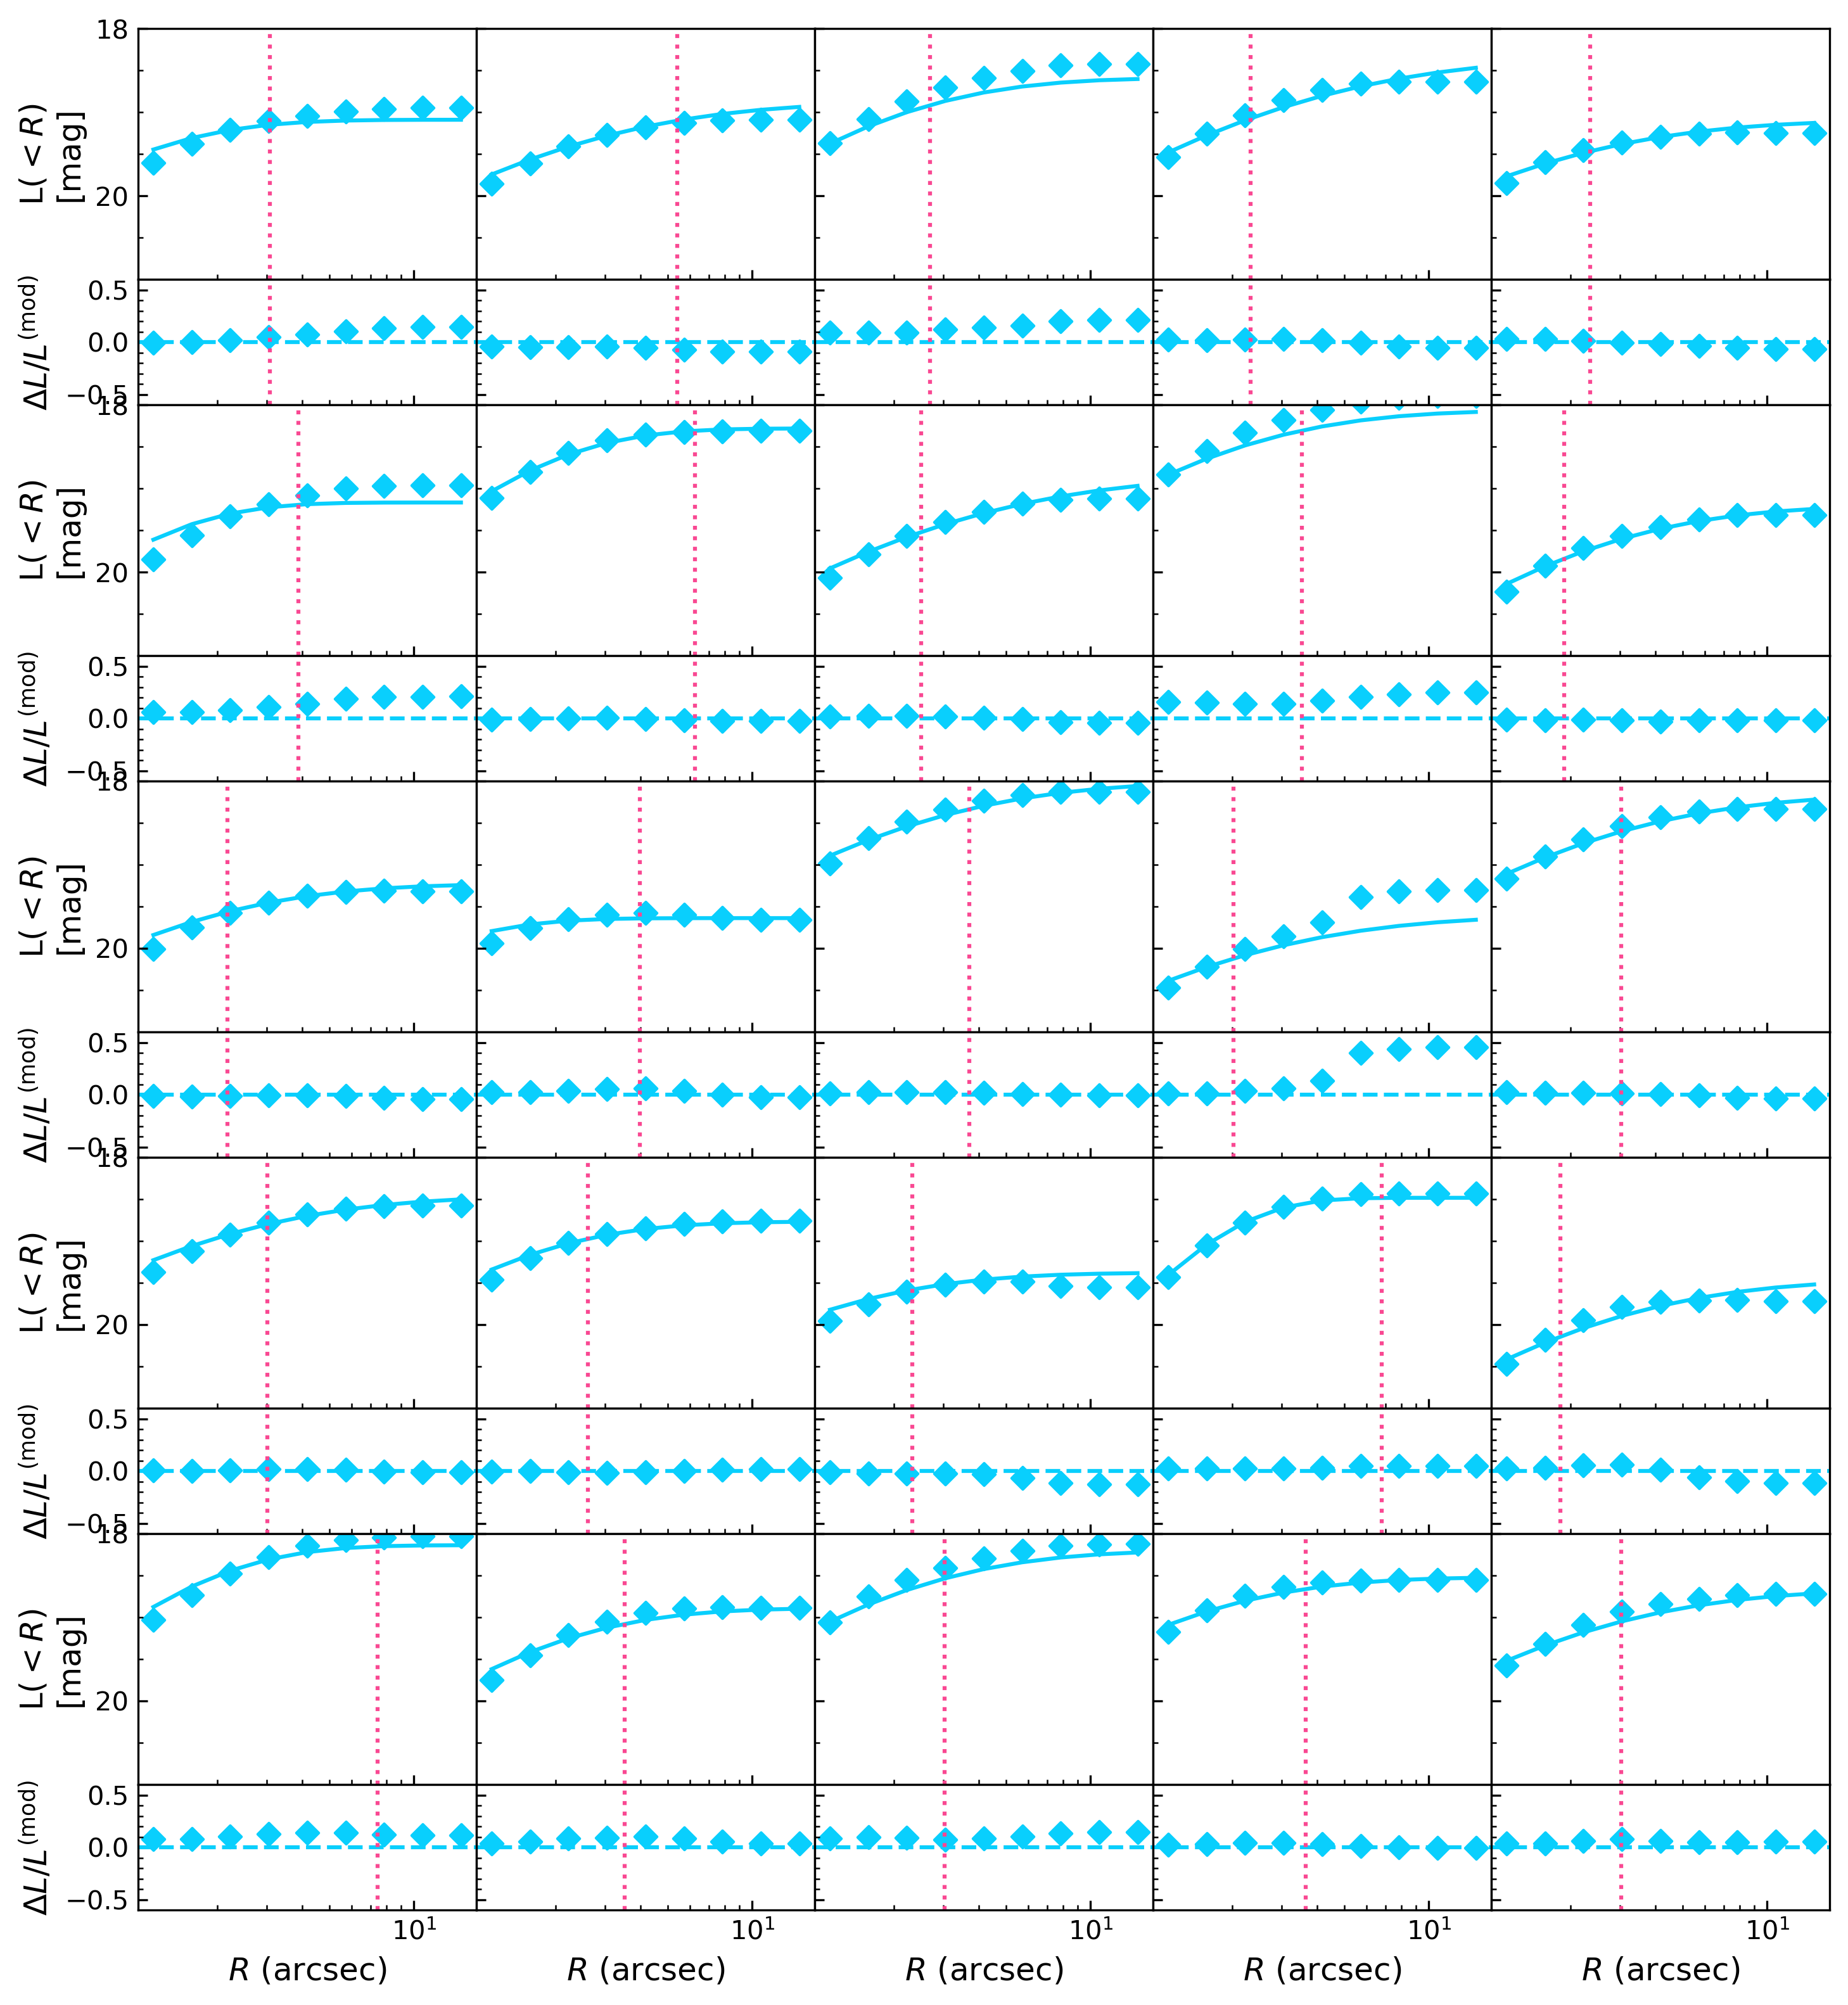
\includegraphics[width=0.8\linewidth]{figure/enclosed_mag.png}
    \caption{The upper panel shows the enclosed magnitude within 10kpc aperture of 25 galaxies that are random selected from our sample. The blue solid line shows the best-fitting S\'{e}rsic model calculated using GalNet structural parameters, while the blue diamonds are directly measured from KiDs r-band image. The lower panel shows the difference between the two measurements. The vertical dashed cyan line shows the corresponding angular size of 10kpc of each galaxy.} 
    \label{fig:enclosed_magnitude}
\end{figure*}
% \subsubsection{Surface brightness model}
% \par Although we have complete the sample with those excluded galaxies, these galaxies are lack of accurate structural parameters. Therefore we need to fit the surface brightness ourselves for those missed galaxies. 
\par The S\'{e}rsic profile can be described by:
\begin{equation}
    I(R) = I_0 exp\left\{-b_n\left(\frac{R}{R_e}\right)^{1/n}\right\}
    \label{SB}
\end{equation}
Here, $q$ is the axis ratio, $n$ is the S\'{e}rsic index while $R$ is the circularised radius
\begin{equation}
    R^2 = qx^2 + \frac{y^2}{q}
\end{equation}
where $x,y$ are Cartesian coordinates, located at the center of galaxies. We use symbol $x$ to denote the axis that is aligned with the semi-major axis of the ellipse, while using $y$ to denote axis aligned with semi-minor axis. The effective radius $R_e$ is circularised as well.
\par Integrating Eq.\ref{SB}, we can obtain the light enclosed in a certain aperture $L(<R)$ 
% (or the total light $L_{tot}$)
\begin{equation}
    \label{eq:light}
    L(<R) = 2\pi n\cdot I_0R_e^2 \cdot \frac{1}{\left(b_n\right)^{2n}}\cdot \gamma\left[2n,b_n \left(\frac{R}{R_e}\right)^{\frac{1}{n}}\right]
\end{equation}
The total light is simply substitute $R = \infty$ to Eq.\ref{eq:light}
\begin{equation}
    L_{tot} = 2\pi n\cdot I_0R_e^2 \cdot \frac{1}{\left(b_n\right)^{2n}}\cdot \Gamma\left(2n\right)
\end{equation}
Here $\Gamma$ is the gamma function, $\gamma$ is the lower incomplete gamma function and $b_n$ is a constant that ensure the light enclosed within the effective radius $R_e$ is a half of the total light.
\begin{equation}
    L_{tot} = 2 L(<R_e)
\end{equation}
Therefore, $b_n$ can be calculated by solving
\begin{equation}
    \Gamma(2n) = 2\gamma(2n, b_n)
\end{equation}

% \par The effective radius provided in fiducial catalogue has already been circularised, while GALFIT actually measured the effective radius $r_e$(use lowercase to denote the value measured by GALFIT) along semi-major axis, hence we need to convert it to circularised radius by 
% \begin{equation}
%     R_e = r_e \times \sqrt{q}
% \end{equation}
% \par We use the sky-subtracted and coadd science image in r-band (in consistent with fiducial sample) and using software SEXTRACTOR(\cite{Bertins_1996_Sextractor}) to mask the neighbouring objects with 1.5$\sigma$ detection threshold. The uncertainty of the sky is provided in the weight image, we then add the poisson noise calculated form the science image in quadruple and thus create the sigma image. We then ran GALFIT(\cite{Peng_galfit_2002}) and obtained S\'{e}rsic parameters for those missed galaxies.
% \par Combining with the S\'{e}rsic fitting result from KiDs DR4 structural catalogue, we obtained a sample within which all galaxies has reliable S\'{e}rsic parameters.We use 'refined sample' to represent this sample. 
\par In our work, we assume that there is no mass-to-light ratio gradient inside one galaxy, hence the mass profile can be easily obtained via the light profile. We have obtained the stellar mass estimate for each galaxy from GAMA together with the light they use in the SPS model fitting process \citep{GAMAmain}, which enable us to calculate the mass-to-light ratio $\Upsilon_*$. The mass profile can be easily obtained by multiplying Eq3 and Eq4 with that $\Upsilon_*$.
\begin{equation}
    \label{eq:sigma}
    \Sigma_*(R) = \Upsilon_* I_0 exp\left\{-b_n\left(\frac{R}{R_e}\right)^{1/n}\right\} 
\end{equation}
\begin{equation}
    \label{eq:mass}
    M_*(<R) = \Upsilon_* 2\pi n\cdot I_0R_e^2 \cdot \frac{1}{\left(b_n\right)^{2n}}\cdot \gamma\left[2n,b_n \left(\frac{R}{R_e}\right)^{\frac{1}{n}}\right]
\end{equation}
Simply substitute $R = 10kpc$ to Eq.\ref{eq:mass}, we obtained $M_{*,10}$, while $\Gamma_{*,10}$ is obtained by substituting Eq.\ref{eq:sigma} to Eq.\ref{eq:gammastar10}.
In fact, we could only obtain the stellar mass estimation from GAMA survey and structure parameter measurement from KiDs survey.As these two surveys may use different aperture size in investigating the same galaxy, these two quantities might not be consistent. Nevertheless, we may make a assumption that the mass-to-light ratio $\Upsilon_*$ do not depend on the distance to the center of galaxy. Therefore, although we could only obtain $\Upsilon_*$ from GAMA survey, we believe it is reasonable to use it to calculate $M_{*,10}$ and $\Gamma_{*,10}$ together with the structure parameter measured by KiDs. 
\par Another concern might arise from the fact that galaxies may have various component, hence single S\'{e}rsic model might not be able to give a accurate description of the entire surface brightness profile. However, as we are focusing on the inner region of the galaxy, our only requirement is just the surface brightness in the inner region of galaxy can be accurately described by model.We compared the profile of the enclosed light of galaxies with their best-fitting S\'{e}rsic model in Fig~\ref{fig:enclosed_magnitude} . We can easily observe that although some model do have discrepancy at some large radii, the enclosed light within $10kpc$ is still well constrained by model. 
% \subsubsection{$M_{*,10}, \Gamma_{*,10}$ Calculation}
% \label{sec:cal}
 
\subsubsection{Completeness}
To accurately measure the evolution of $M_{*,10}$ and $M_{*,10} - \Gamma_{*,10} $ relation, we do not expect any bias be introduced during the sample selection procedure. Therefore, we need our sample to be complete in $M_{*,10}$. Our fiducial sample is flux-limited, with its 95\% completeness limit down to r-band magnitude 19.65. To obtain a $M_{*,10}$ complete sample, we need to translate this completeness limit in magnitude to limit in $M_{*,10}$.
% \par GAMA provide the stellar mass estimation together with the r-band flux from SPS fit in its stellar mass DMU(\cite{GAMAmain}). We hence calculate the fraction of these two value and obtain the mass-to-flux ratio $\Upsilon$. Then we use the S\'{e}rsic parameters($R_e,n,b_n$) and the magnitude from surface brightness fitting in our refined sample  and calculated the flux that is enclosed in 10kpc $F_{10}$. It's straightforward that we can just multiply these two quantities and get $M_{*,10} = \Upsilon \times F_{10}$.
\par Then we need to translate the r-band critical magnitude $r_{crit} = 19.65$ to one critical $M_{*,10}$, namely $M_{*,10}^{crit}$. In fact, at a given redshift, the ratio between $M_{*,10}$ and the total flux $F$ always spread a relatively wide range. Here we made an assumption that the ratio $M_{*,10} / F$ depend neither on $M_{*,10} $ nor on $F$, meaning that this quantity only describe one overall nature of quiescent galaxies at one given redshift. We then make narrow redshift bins, measure the distribution of $M_{*,10} / F$ in each bin and find the critical value $M_{*,10} / F|_{crit}$
% calculate the mean and standard deviation of the mass-to-flux ratio $M_{*,10} / F$ and use Gaussian distribution to estimate the critical value $M_{*,10} / F|_{crit}$
 ,where the cumulative probability reach $95\%$ .Multiplying $M_{*,10} / F|_{crit}$ by the corresponding flux of $r_{crit}$, we obtained the $M_{*,10}$ limit at that redshift bin. 
\begin{figure}
    \centering
    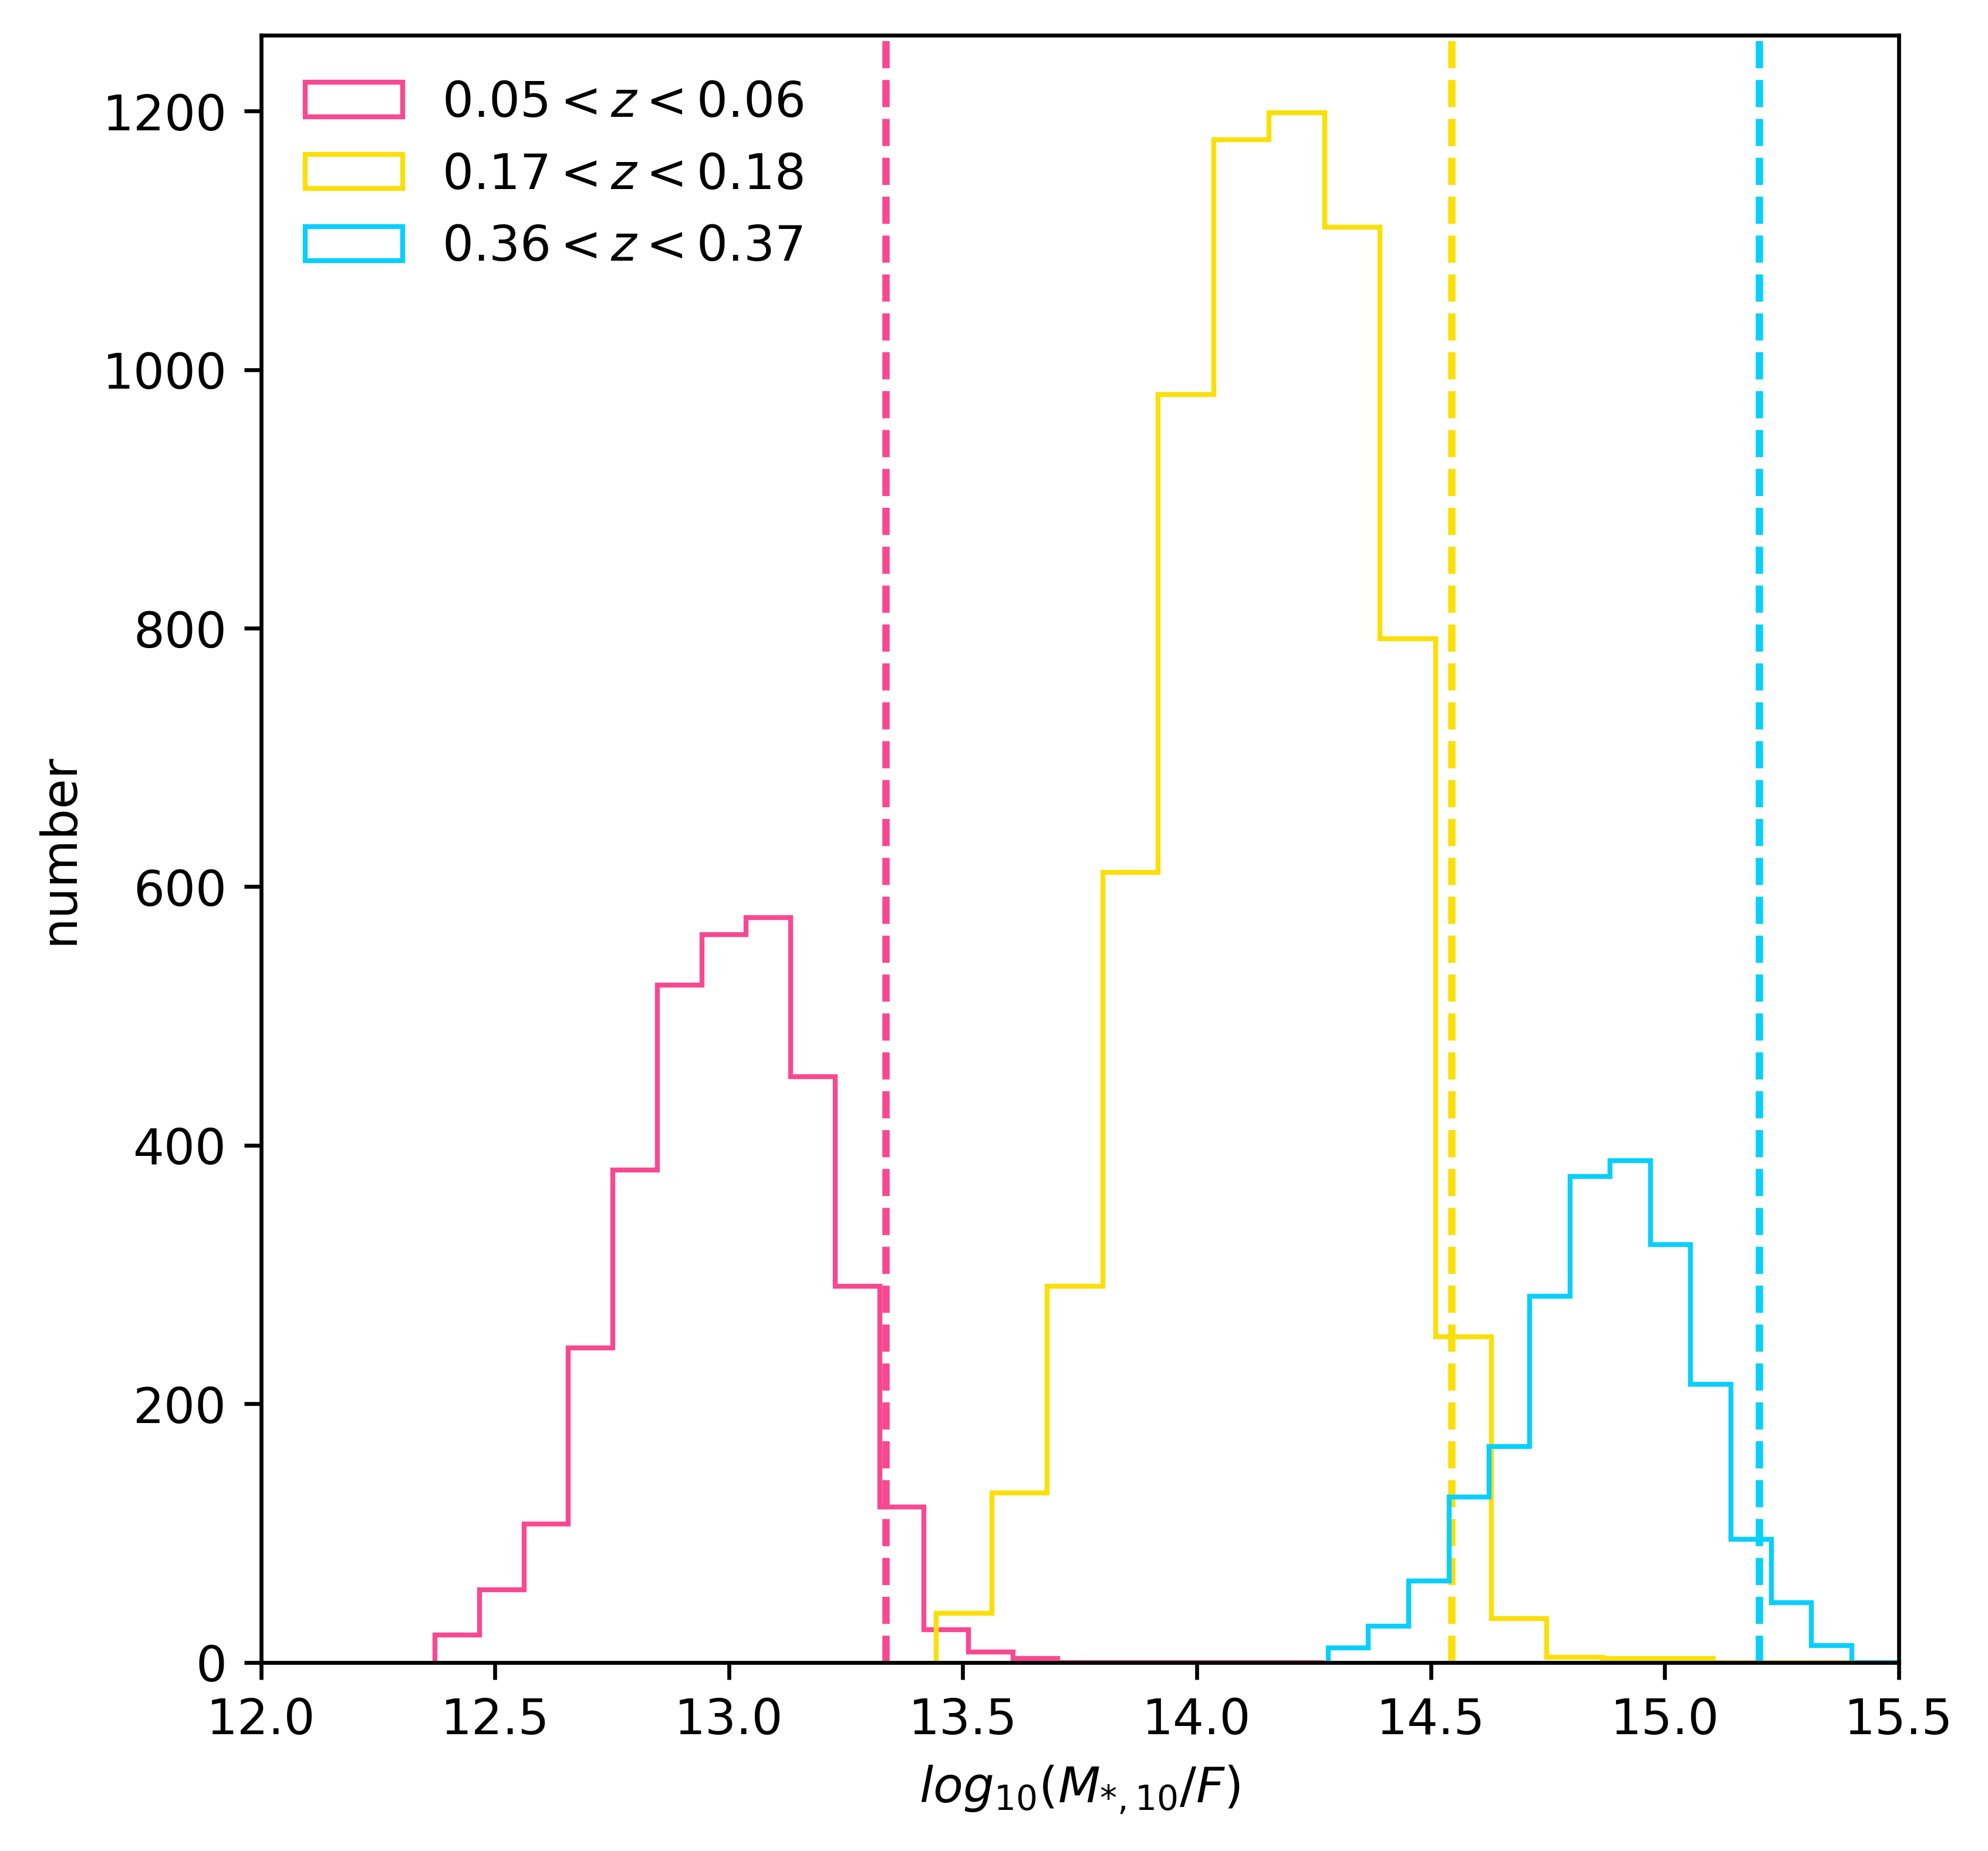
\includegraphics[width=\linewidth]{figure/m2f_ratio.png}
    \caption{The distribution of $M_{*,10} / F$ in three different narrow redshift bins. The vertical dashed line marks the $95\%$ percentile distribution in each bin.Multiply this ratio by the flux corresponding to the r-band magnitude limit $r_{crit} = 19.65$, we then obtain the $M_{*,10}$ limit at that redshift bin.}
    \label{fig:m2f}
\end{figure}
\par Fig~\ref{fig:m2f} illustrate the procedure, here we randomly choose three different redshift bins and shows the distribution of $M_{*,10} / F$ inside, with dashed line showing the $95\%$ percentile of each bin, i.e. the critical mass-to-flux ratio $M_{*,10}/F|_{crit}$. The flux correspond to r-band magnitude $19.65$ is $F_{crit} \approx  5.01 \times 10^{-5} \text{Jy} $.The $M^{crit}_{*,10} $ in this three bins can thus by $M^{crit}_{*,10} = M_{*,10}/F|_{crit} \times F_{crit} $ using the value of $M_{*,10}/F|_{crit}$ in each bins.  Operate this procedure iteratively in each redshift bin result in the full $95\%$ completeness limit in $M_{*,10}$ as a function of redshift $z$ . In addition, we use a exponential formula to fit this limit
\begin{equation}
    f(z) = A(z+B)^C + D
\end{equation}
the best-fitting parameter are shown in 
\begin{table}
    \centering
    \caption{The best-fitting parameter of the exponential function that describe the $95\%$ completeness limit in $M_{*,10}$ as a function of redshift.}
    \label{tab:completeness}
    \resizebox{\columnwidth}{!}{
    \begin{tabular}{cccc}
        \hline
        A & B & C & D \\
        \hline
        $8.34  \times 10 ^3$ &$ 9.71 \times 10^{-4}$ &$ 1.06 \times 10^{-4}$ & $-8.3 \times 10^{3}$ \\
        \hline
    \end{tabular}}
\end{table}
\par Fig~\ref{fig:completeness_cut} shows the distribution of our sample in $M_{*,10} - z$ space, with the pink solid line shows the $95\%$ completeness limit. We think galaxies whose $M_{*,10}$ is larger than the limit is $95\%$ possible to be included in our fiducial sample. We thus exclude those galaxies whose $M_{*,10}$ is lower than this limit in our fiducial sample and show these galaxies in grey dots. Galaxies shown in black dots are included to built our complete sample.
 Actually, we use the galaxies that are shown in cyan dots in this figure to investigate the evolution of $\Gamma_{*,10}$ and $M_{*,10} - \Gamma_{*,10}$ relation, as described in Sect.\ref{sec:obres}.
\begin{figure}
    \centering
    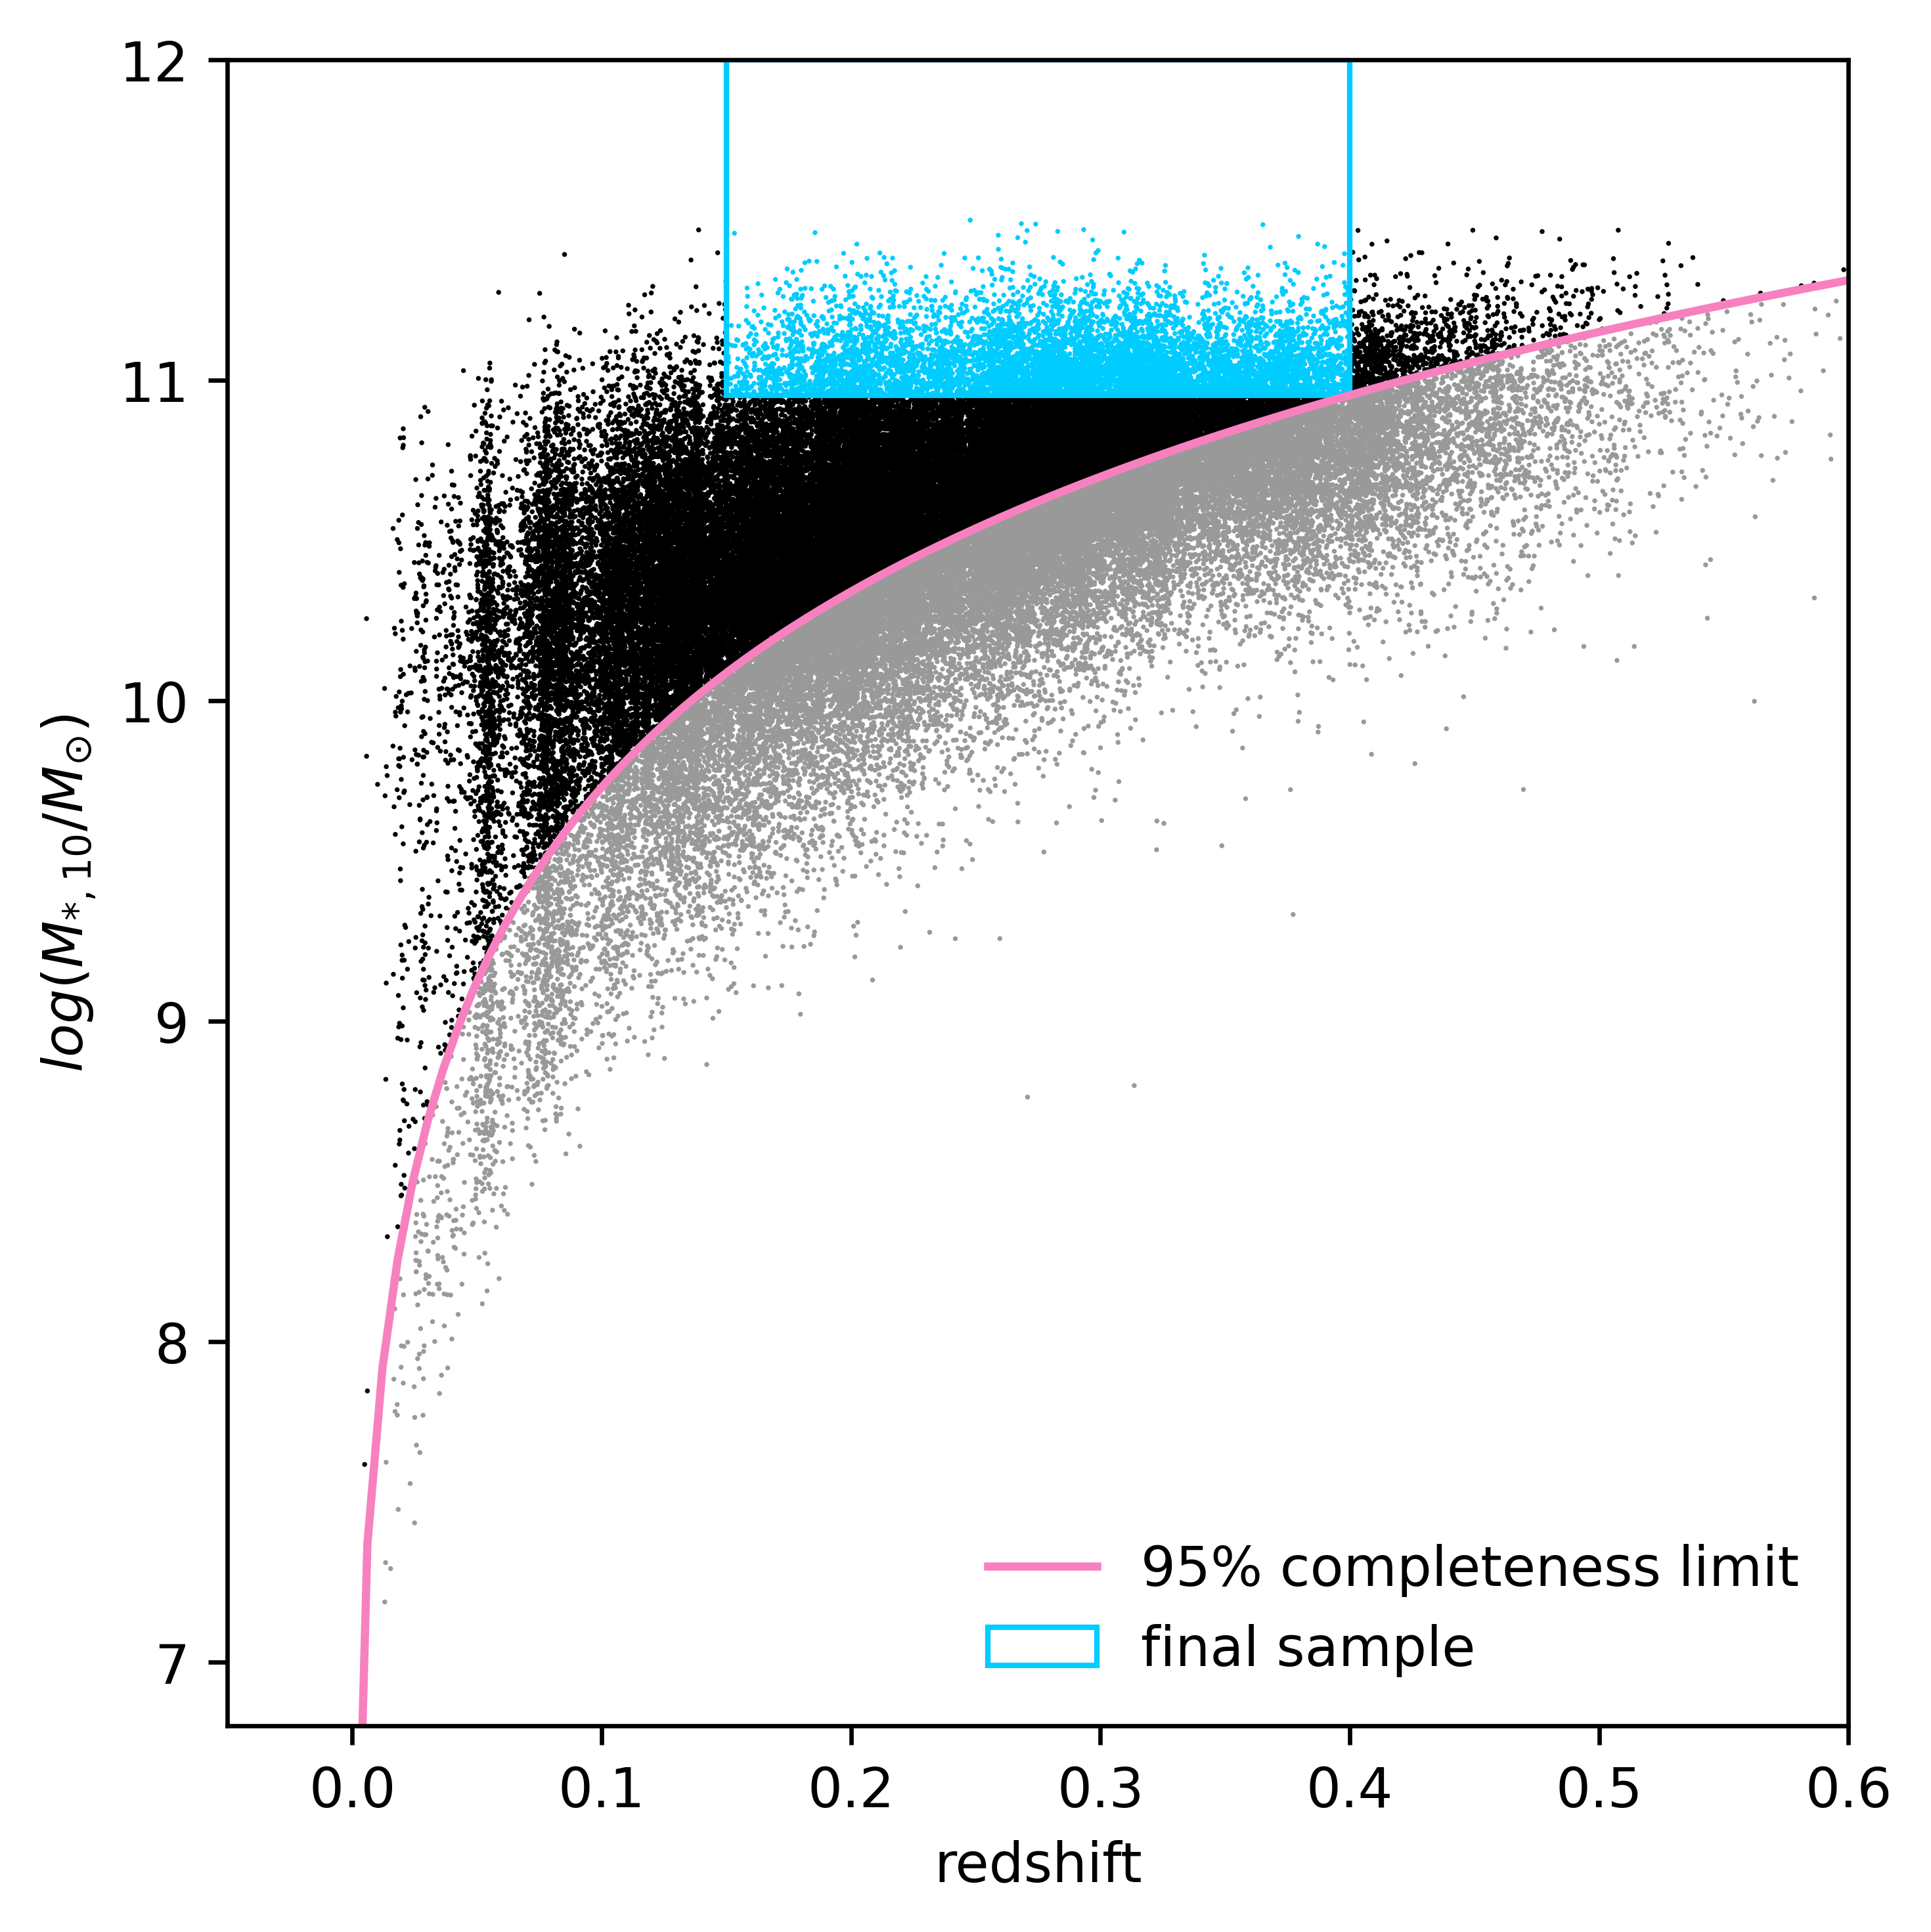
\includegraphics[width = \linewidth]{figure/completeness_cut.png}
    \caption{$95 \% $ completeness $M_{*,10} $ limit as a function of redshift of our ETG sample, shown in pink solid line.Galaxies above this pink line is adopted in our sample, shown in black dots, and the grey dots that lies below are those being excluded  }
    \label{fig:completeness_cut}
\end{figure}
% \par According to \cite{gallazzi_stellarmass_2009}, red galaxies has much narrower distribution of mass-to-light ratio than the blue one, hence the distribution of those red galaxies would be truncated at some stellar mass and the low mass end would be dominated by blue galaxies. This two population will mix with each other at higher stellar mass, exhibiting a nearly uniform color distribution. In Fig~\ref{fig:completeness_cut}, we can observe that our completeness has avoided those region that dominated by blue galaxies and selected the mixture of red and blue galaxies.
% In this paper, one basic assumption is the mass-to-light ratio is constant at arbitrary position of one galaxies.

% then used GALFIT(\cite{Peng_galfit_2002}) to fit a seeing convolved S\'{e}rsic model for those galaxies using r-band photometry. Neighbouring galaxies are masked using SEXTRACTOR (\cite{Bertins_1996_Sextractor})
% \subsection{GAMA Spectroscopy}
% In this work, we choose galaxies from GAMA DR4\citep{GAMAmain} with $Dn4000 > 1.5$, in order to choose ETGs, and then we've done a crossmatch with kiDs data. Given that the stellar-mass measurement of KiDs uses photometric redshift, we make use of the stellar mass catalogue provided by GAMA. We calculate the ratio between stellar mass and the derived r-band flux from the SPS fitting. We further assumed the "mass-to-flux" ratio is constant in a single galaxy, then we can use this value to calculate the stellar mass using the photometric data, specifically the r band magnitude, of KiDs'. 
% \par According to GAMA DR4\citep{GAMAmain}, the completeness of galaxies is less than $95\%$ for galaxies with r-band magnitude greater than $19.8$. We desire a complete sample in stellar mass, so we investigate the distribution of stellar mass in each redshift range with r-band magnitude equals to 19.8, in order to convert the completeness in magnitude to the completeness in stellar mass. The distribution is shown in figure 1. In various redshift, we find the stellar mass corresponding to the 95 percentile of the distribution and exclude the galaxies with lower stellar mass value.  

% \subsection{KiDs}
% In this work, we use the “2DPHOT structure parameter catalogue" in DR4-KiDs-1000(We'm not sure which paper to cite). After cross-matched with GAMA data, we first convert the r-band magnitude provided by this catalogue to the flux data. Then we use the "mass-to-flux" ratio calculated using GAMA data and obtain the self-consistent stellar mass for KiDs photometric data. 
% \par In addition to the photometric data, the catalogue also provided the Serisic parameters of each galaxy. Using these parameters, we are able to construct the surface brightness profile by
% \begin{equation}
%     We(R) = I_0exp\left \{-b(n\left(\frac{R}{R_e}\right)^{1/n}\right\}
% \end{equation}
% \par Here $R$ is the circulised radius $R^2 \equiv qx^2+ \frac{y^2}{q}$, where $q$ is the axis ratio. The "structure catalogue provided us the half-light radius $R_e$ and the S\'{e}rsic index $n$.$I_0$ is the surface brightness in the center of one galaxy and $b(n)$ can be calculated by constraining the region enclosed in the hald-light radius $R_e$ contains half of the total light.Hence, we can calculate the mass enclosed in $10kpc$($M_{*,10}$) and the mass-weighted projected surface brightness slope ($\Gamma_{*,10}$)
% \subsection{Completeness}
\subsection{$M_{*,10}$ - $\Gamma_{*,10}$ relation}
As a consequence of the completeness cut, galaxies with lower $M_{*,10}$ value at higher redshift would be absent in our sample. To investigate the evolution trend in $M_{*,10 } - \Gamma_{*,10}$ relation, we have to either narrow the redshift range to include more low-$M_{*,10}$ galaxies or narrow the $M_{*,10}$ range to include more high-redshift galaxies. In this work, we choose the latter one, meaning that we only focus on massive quiescent galaxies whose $M_{*,10} \geq 10^{10.9} M_{\odot}$. In addition, we set a lower limit on the redshift range $ z \geq 0.15$. It's easy to observe some vertical stripe-like feature in Fig.\ref{fig:completeness_cut} at low redshift end, and is thought to be the effect of large scale structure by \cite{GAMAmain}. It is reasonable as the comoving volume at low redshift is relatively smaller, so it is more likely to suffer from cosmic variance. We thus determined this low-redshift cut in order to avoid such cosmic variance. The final sample we used to investigate the evolution is show by cyan dots in Fig.\ref{fig:completeness_cut}. We further separate the sample into four different redshit bins.  
\par In order to infer the distribution of $\Gamma_{*,10}$ as a function of $M_{*,10}$ in different redshift bins, we use a Beyesian hierarchical method to do the fitting. Each galaxy included in our sample can be described by a set of quantities $\{ \log M_{*,10}, \Gamma_{*,10}, z \}$. The true value of these quantities, hereafter represented by $\mathbf{\Theta}$, are drawn from a probability distribution that correlated with the observed data $\mathbf{d} = \{ \log M_{*,10}^{obs}, \Gamma_{*,10}^{obs}, z^obs \}$, and is in turn described by a set of hyperparameters $\mathbf{\Phi}$.We expect to obtain the posterior distribution of the hyperparameters $\mathbf{\Phi}$ given the observed data $\mathbf{d}$: 
\begin{equation}
    P(\mathbf{\Phi}|\mathbf{d}) \propto  P(\mathbf{\Phi}) P(\mathbf{d}|\mathbf{\Phi})
\end{equation}
thus we marginalize every possible value of $\mathbf{\Theta}$ in the likelihood part: 
\begin{equation}
    \label{Eq:likelihood}
    P(\mathbf{d}|\mathbf{\Phi}) = \int P(\mathbf{d}|\mathbf{\Theta})P(\mathbf{\Theta}|\mathbf{\Phi})d\mathbf{\Theta}
\end{equation}
\par As we hope to acquire the $\Gamma_{*,10} -M_{*,10}$  relation, we may rewrite the second part on the R.H.S. of Eq.\ref{Eq:likelihood} as
\begin{equation}
    P(\mathbf{\Theta}|\mathbf{\Phi}) =  P(\log M_{*,10}|\mathbf{\Phi})P(\Gamma_{*,10}|\mathbf{\Phi},\log M_{*,10})
\end{equation}
Note that we have binned the sample into four different redshift bins, hence we ignore the redshift dependence of the hyperparameters $\mathbf{\Phi}$.
\par  For the distribution of $\log M_{*,10}$, we use a skew normal distribution to describe : 
\begin{small}
   \begin{equation}
        P\left(\log M_{*,10}|\Phi\right) = \frac{1}{\sqrt{2\pi\sigma^2_M}}exp\left\{-\frac{(\log M_{*,10} - \mu_M)^2}{2\sigma_M^2}\right\}\mathcal{E}\left(\log M_{*,10} | \Phi\right)
    \end{equation} 
\end{small}
where
\begin{equation}
    \mathcal{E}\left(\log M_{*,10} | \Phi\right) = 1 + erf\left(\alpha_M\frac{\log M_{*,10} - \mu_M}{\sqrt{2\sigma_M}}\right)
\end{equation}
In fact, having considered the $\log M_{*,10}$ distribution, our model are automatically corrected the so called Eddington bias. 
\par For the distribution of $\Gamma_{*,10}$, we use a Gaussian distribution to describe:
\begin{equation}
    P\left(\Gamma_{*,10}|\Phi,\log M_{*,10}\right) = \frac{1}{\sqrt{2\pi\sigma^2_{\Gamma}}}exp\left\{-\frac{(\Gamma_{*,10} - \mu_{\Gamma})^2}{2\sigma_{\Gamma}^2}\right\}
\end{equation}
The relation between $\log M_{*,10}$ and $\Gamma_{*,10}$ is described by the $\log M_{*,10}$ dependence on $\mu_\Gamma$:
\begin{equation}
    \label{eq:mg_relation}
    \mu_{\Gamma} = \mu_{\Gamma,0} + \mu_{\Gamma, ms}\left(\log M_{*,10} - \log M^{piv}_{*,10}\right)
\end{equation}
Here we use a pivot value for $\log M_{*,10}$, which is the median value in each redshift bins.
\par Therefore, the full distribution of $\Theta$ given $\mathbf{\Phi}$ is governed by the following set of hyperparameters:
\begin{equation}
    \mathbf{\Phi} = \{ \mu_M, \sigma_M, \alpha_M, \mu_{\Gamma,0}, \mu_{\Gamma, ms}, \sigma_{\Gamma} \}
\end{equation}
\par For the first part on the R.H.S. of Eq.\ref{Eq:likelihood}, we may rewrite it as
\begin{equation}
    P(\mathbf{d}|\mathbf{\Theta}) = P(\log M^{obs}_{*,10}|\log M_{*,10})P(\Gamma^{obs}_{*,10}|\Gamma_{*,10})P(z^{obs}|z)
\end{equation}
\par Fortunately, according to Eq.\ref{eq:gammastar10},Eq.\ref{eq:sigma}and Eq.\ref{eq:mass}, the uncertainty of $\Gamma_{*,10}$ has cancelled out. In addition, as we use spectroscopic redshift, the uncertainty of $z$ is negligible. Therefore, we only need to consider the uncertainty of $\log M_{*,10}$, which we assume can be described by a Gaussian distribution:
\begin{tiny}
    \begin{equation}
        P[\log (M_{*,10}^{obs})|\log (M_{*,10})] = \frac{\mathcal{A}[\log (M_{*,10})]}{\sqrt{2\pi\sigma^2_{M_{*,10,obs}}}}exp\left\{-\frac{[\log (M_{*,10}) - \log (M_{*,10}^{obs})]^2}{2\sigma_{M_{*,10, obs}}^2}\right\}
    \end{equation}
\end{tiny}
while $\mathcal{A}[\log (M_{*,10})]$ satisfies
\begin{tiny}
    \begin{equation}
        \int_{log(M_{*,10,min})}^\infty dlog(M_{*,10}^{obs})\frac{\mathcal{A}[log(M_{*,10})]}{\sqrt{2\pi\sigma^2_{M_{*,10,obs}}}}exp\left\{-\frac{[log(M_{*,10}) - log(M_{*,10}^{obs})]^2}{2\sigma_{M_{*,10, obs}}^2}\right\} = 1 
    \end{equation}
\end{tiny}
\par We sampled the posterior distribution of these hyperparameters and find the median value . The result is shown in Table.\ref{tab:mg_relation}. 
\begin{table}
    \renewcommand\arraystretch{1.5}
    \centering
    \caption{Beyesian hierarchical model fitting for the $\Gamma_{*,10} - M_{*,10}$ relation in different redshift bins.}
    \label{tab:mg_relation}
    \resizebox{\columnwidth}{!}{
    \begin{tabular}{ccccccc}
        \hline
        redshift & $\mu_M$ & $\sigma_M$ & $\alpha_M$ & $\mu_{\Gamma,0}$ & $\mu_{\Gamma, ms}$ & $\sigma_{\Gamma}$ \\
        \hline
        0.15-0.21 & 10.92 & 0.16 & 6.34 & $1.51^{+0.003}_{-0.003}$ & $-0.34^{+0.04}_{-0.04}$ & 0.10 \\
        0.21-0.28 & 10.94 & 0.15 & 4.34 & $1.52^{+0.003}_{-0.003}$ & $-0.38^{+0.03}_{-0.03}$ & 0.10 \\
        0.28-0.34 & 10.89 & 0.16 & 20.07 & $1.51^{+0.002}_{-0.002}$ & $-0.38^{+0.03}_{-0.03}$ & 0.10 \\
        0.34-0.40 & 10.89 & 0.15 & 2.09 & $1.50^{+0.003}_{-0.003}$ & $-0.23^{+0.03}_{-0.03}$ & 0.11 \\
        \hline
    \end{tabular}}
\end{table}
In addition, to illustrate the $\Gamma_{*,10}$ - $M_{*,10}$ relation, which is decribed by Eq.\ref{eq:mg_relation}, we plot $\mu_\Gamma$ as a function of $\log M_{*,10}$ in Fig.\ref{fig:mg_relation} in dotted line, while the shaded region represent $68\%$ credible interval of the distribution. 
\par We could observe an anit-correlation between $\Gamma_{*,10}$ and $M_{*,10}$, which is qualitatively in agreement with traditional $R_e - M_*$ scaling relation. Galaxies with larger stellar mass tend to have larger size, i.e. larger $R_e$, and hence the surface mass profile would decrease slower and have a smaller $\Gamma_{*,10}$. The relation in the highest redshift bin shows a significant difference comparing with the other three bins, either in the slope or in the normalization. The other three redshift bins, however, could be considered as in broad agreement within $1 \sigma$ level. This feature might indicate that quiescent galaxies do grew in the redshift range that we focus, but we are still not clear what could be the mechanism behind the growth. Therefore, we utilized a binary merger simulation and tried to establish a toy model built upon the 'minor merger' scenario to predict the variation in $\Gamma_{*,10}- M_{*,10}$ relation.The details are shown in the following section. 
\begin{figure}
    \centering
    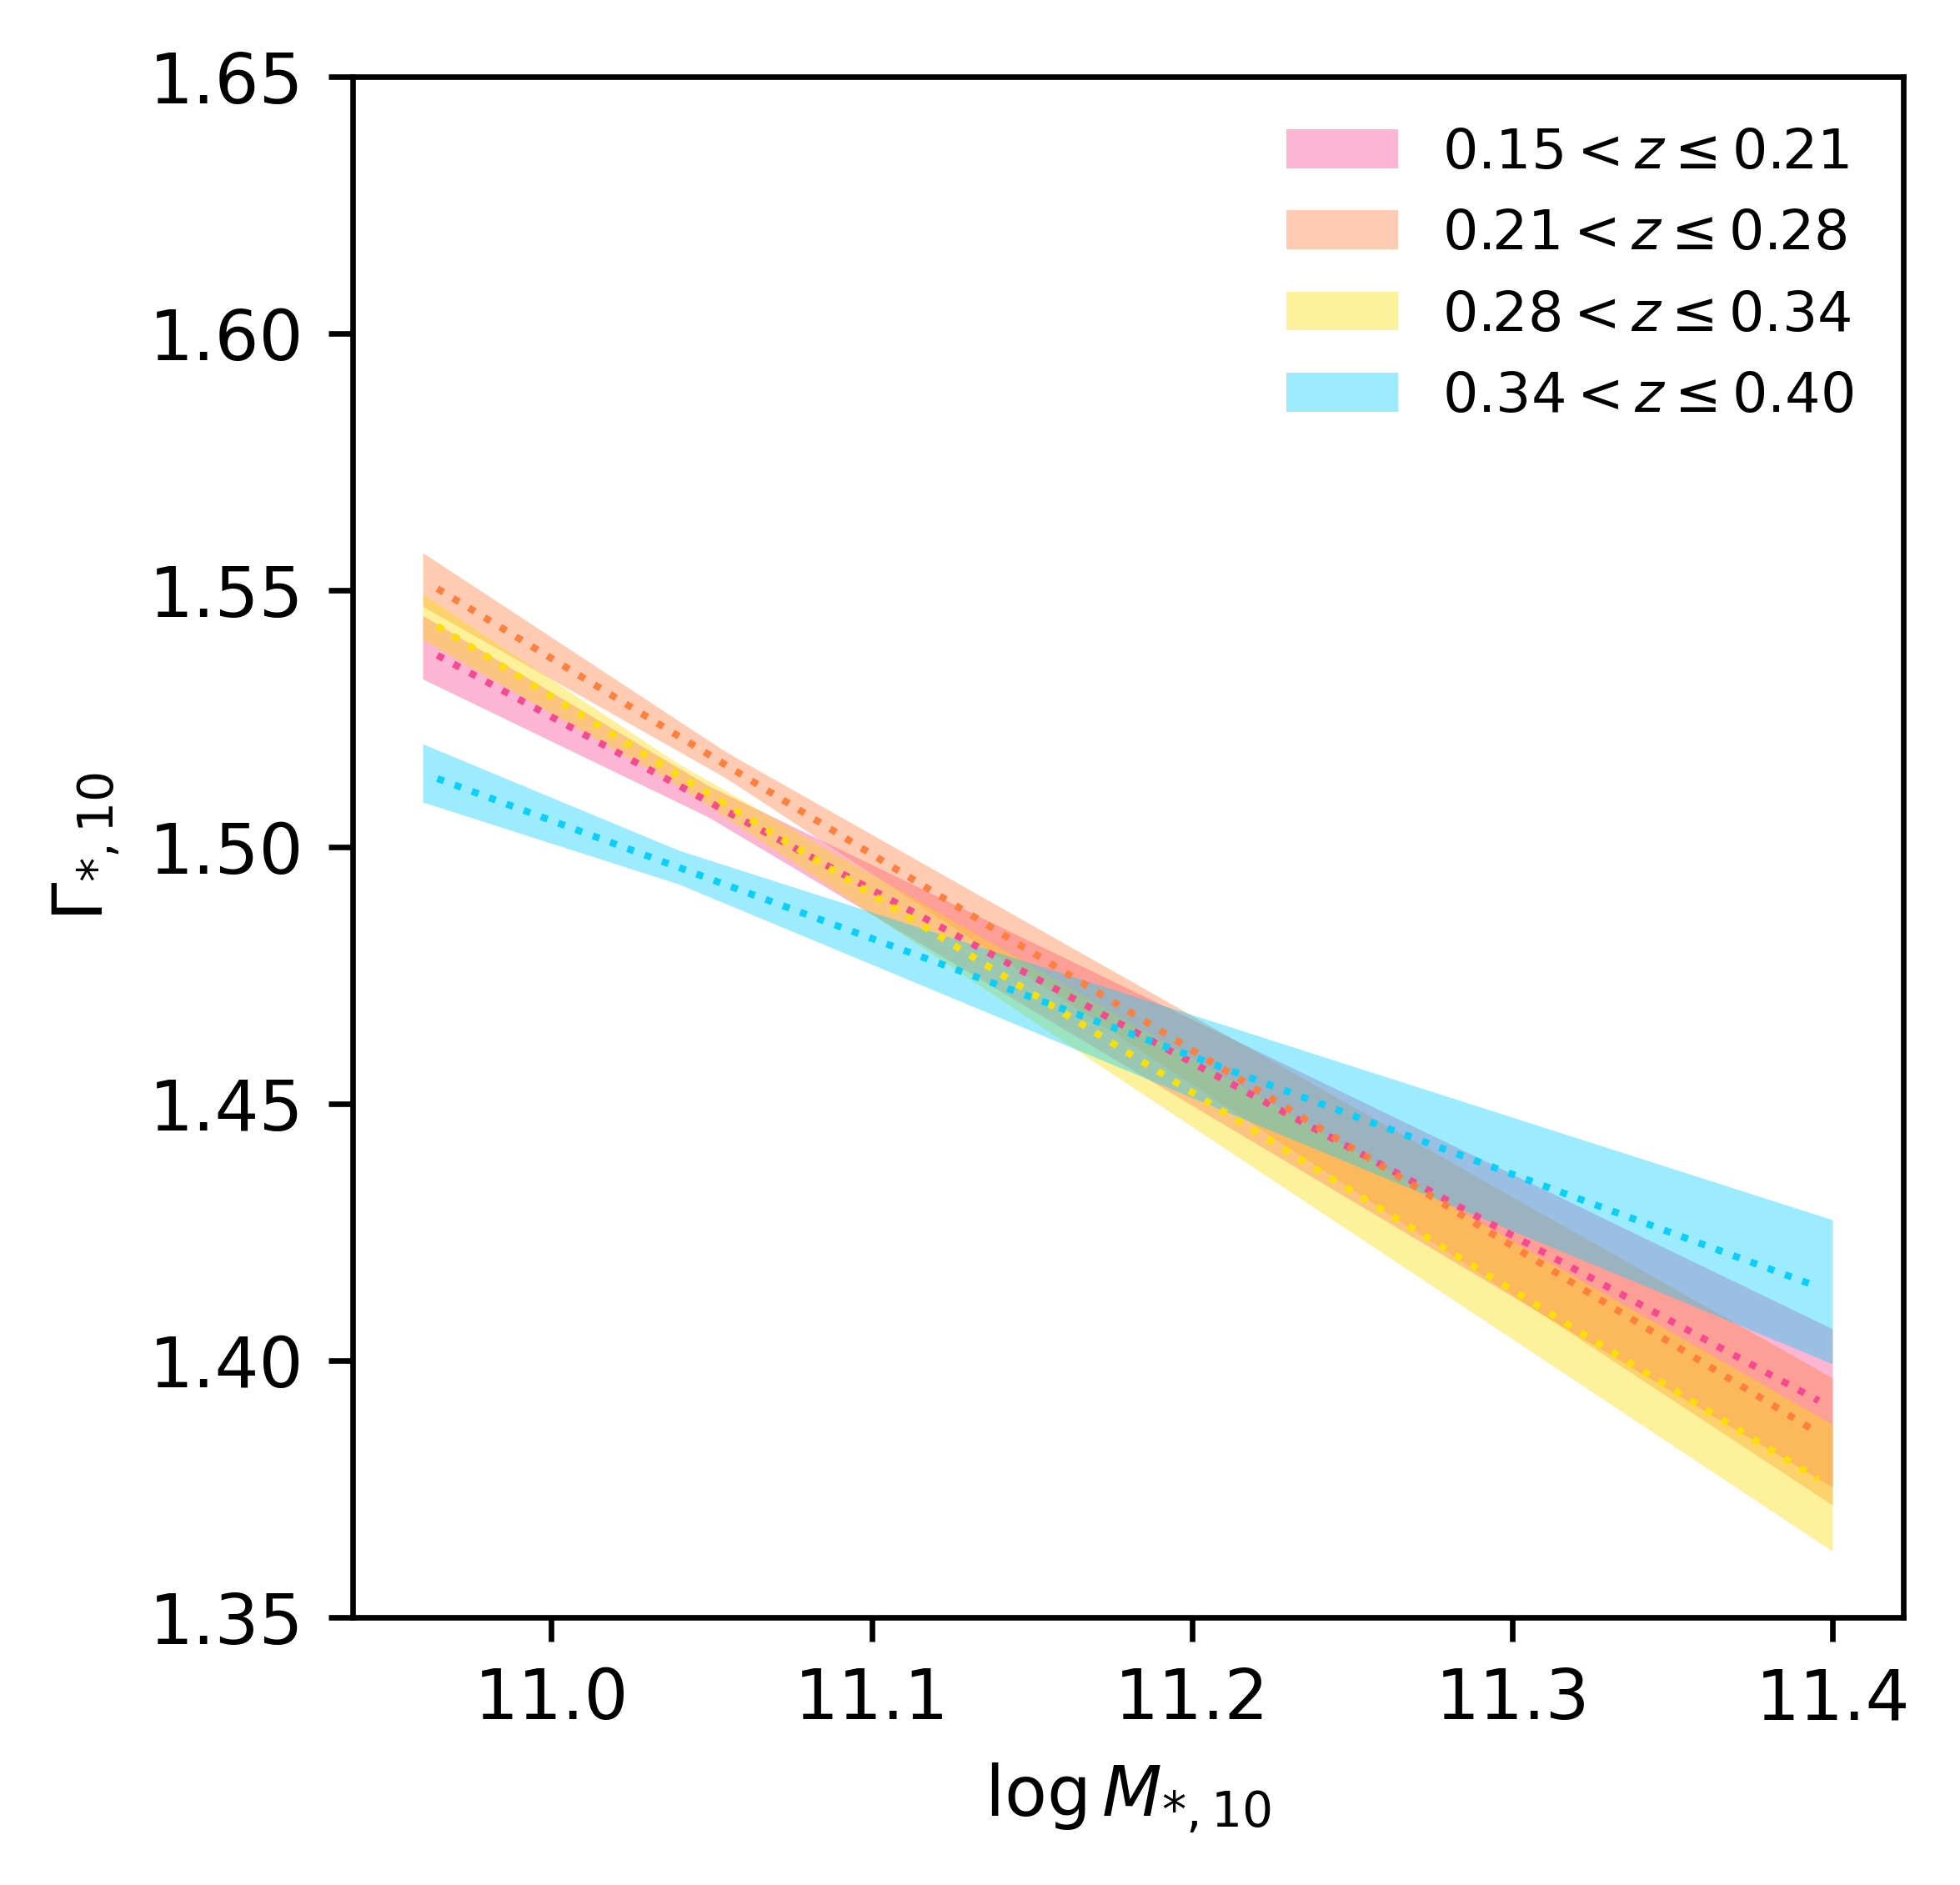
\includegraphics[width=\linewidth]{figure/mg_relation.png}
    \caption{The $M_{*,10} - \Gamma_{*,10}$ relation of our observation sample. The sample are divided into four redshift bins, and are shown in different colors. The error bar represents the standard error in each bins.}
    \label{fig:mg_relation}
\end{figure}
\section{Simulation}
\label{sec:3}
\subsection{Data set}
\subsubsection{Basic information}
As mentioned in Sect.\ref{sec:intro}, we expect to understand how mergers, in particular, dry mergers with different merger mass ratio, would affect $M_{*,10}$ and $\Gamma_{*,10}$. 
Therefore, we utilize a collection of 8 sets dissipationless binary-merger simulations which has been used in \cite{sonnenfeld2014} to construct a dry-merger model. These 8 sets of simulations has five different parameter settings and is reported in Table~\ref{tab:simulation}. 
Each set contains two runs of simulations with nearly identical parameter settings except for their different orbital angular momentum in order to take both 'head-on' and 'off-axis' encounter into consideration. All orbits are parabolic.   
\begin{table}
    \renewcommand\arraystretch{1.5}
    \centering
    \caption{Simulation parameters for different sets of simulation. }
    \label{tab:simulation}
    \resizebox{\columnwidth}{!}{
    \begin{tabular}{cccccccc}
        
        \hline
        % \hline
        Set & $\xi$ & $(M_h/M_*)_{\text{main}}$ & $C_{\text{main}}$ & $(r_s/R_{\text{eff}})_{\text{main}}$ & $(M_h/M_*)_{\text{sat}}$ & $C_{\text{sat}}$ & $(r_s/R_{\text{eff}})$ \\
        \hline
        D & 1.0,0.5,0.2 & 49 & 8.0 & 11.6 & 49 & 8.0 & 11.6 \\
        D1 & 0.5 & 49 & 5.0 & 11.6 & 49 & 5.0 & 11.6 \\
        D2 & 0.5 & 49 & 8.0 & 6.0 & 49 & 8.0 & 6.0 \\
        D3 & 0.2 & 49 & 8.0 & 11.6 & 35 & 8.5 & 8.8 \\
        D4 & 0.2 & 49 & 8.0 & 11.6 & 75 & 8.0 & 15.0 \\
        \hline
    \end{tabular}}
\end{table}
\par The two progenitors, i.e. main galaxy and satllite galaxy , in each set of simulation are spherical symmetric and are composed of dark matter halo and stellar component. The stellar profile can be decribed by $\gamma$ model (\cite{Dehnen93}; \cite{Tremaine94})
\begin{equation}
    \label{eq:profile_stellar}
    \rho_*(r) = \frac{3-\gamma}{4\pi}\frac{M_*r_*}{r^\gamma (r+r_*)^{4-\gamma}}
\end{equation}  
where $M_*$ is the total stellar mass. The simulation adopt $\gamma = 1.5$ . 
\par The dark matter halo is described by NFW profile (\cite{NFW})
\begin{equation}
    \label{eq:profile_halo}
    \rho_{DM}(r) = \frac{M_{DM,0}}{r(r+r_s)^2} exp\left[-\left(\frac{r}{r_{vir}}\right)^2\right]
\end{equation}
According to \cite{nipoti2009}, $r_s$ is the scale radius, while $M_{DM,0}$ is a reference mass. A exponential cut-off is adopted as a truncation of the halo, hence the total dark mass would not extend to infinity. As the summation of the two components, the total mass profile $\rho(r) = \rho_*(r) + \rho_{DM}(r)$ is nearly isothermal: the slope $\gamma'$ of the toal mass profile in 8 sets of simulation lies in the range of $1.97 \sim 2.03$.

\par The simulation is run with FVFPS code (Fortran Version of Fast Poisson Solver, \cite{londrillo03,nipoti03}) The following code parameter values are adopted: minimum value of the opening parameter $\theta_{min} = 0.5$ while the softening parameter $\epsilon = 0.04 R_\text{eff}$, here $R_\text{eff}$ represent the effective radius of the main galaxy. The timestep $\Delta t$ is the same for all particles, while is allowed to vary depending on the maximum particle density $\rho_{max}$ at that epoch.In particular, the timestep can be adapted by $\Delta t = 0.3/(4\pi G \rho_{max})^{1/2}$.The realisation of the initial condition is identical to that in \cite{nipoti2009}, with the mass of dark matter parts twice as heavy as stellar particles.
\subsubsection{Mock observation}

% \par As the origin simulation data didn't give a physical unit of both mass and radius, we now have the freedom to 'rescale' the simulation data to generate galaxies with different size and mass. In practise, we modify the remnant galaxy with three different length unit so that the effective radius $R_e$ of the remnant galaxy equals to $1.22,5,10 kpc$.  
% \section{Method}
% \subsection{Random catalogue}
% Obtaining the $M*_{,10}$ and $\Gamma_{*,10}$ data, we want to plot the $M_{*,10}$ function and investigate its redshift-dependent evolution ,which require us to know the effective volume of our sample. Here we apply the random catalogue method to investigate such issue........
% \subsection{Beyesian hierarchical method?}


In order to investigate the growth of these two parameters, we only need to focus on two snapshots of the simulation. The first snapshot is the initial state which contains the initial main galaxy and satellite galaxy, in fact, we only care about the main galaxy. The second snapshot is the final state when the merging process is finished leaving a remnant galaxy. The word 'finish' means that the remnant stellar system is relaxed and virialised, while the remnant galaxy is denfined as the collection of dark matter particles and stellar particles that are bounded. We project the initial and remnant galaxies onto x-y plane so as to generate a mock observational image of these two, the mock image is shown in Fig.\ref{fig:mock_image}.The initial main galaxy is spherical, thus its image is a circle. In contrast, the remnant galaxy does not have this symmetry, hence we can observe that its image is a ellipse. In order to make a fair comparison, we then circularised the remnant ellipse. In particular, we measured the quadruple moment of the remnant galaxy image, and then stretch and rotate the image according to this quadruple moment until the image become a circle.
\begin{figure*}
    \centering
    \includegraphics[width=\linewidth]{figure/circularised.png}
    \caption{\label{fig:mock_image}In this plot We choose the simulation set D3 to illustrate the mock images of main and remnant galaxies. The left panel shows the  initial main galaxy, while the middle and right panels are  the uncircularised and circularised remnant galaxy respectively. The unit is in code unit, instead of physical unit}
\end{figure*}
\begin{figure}
    \centering
    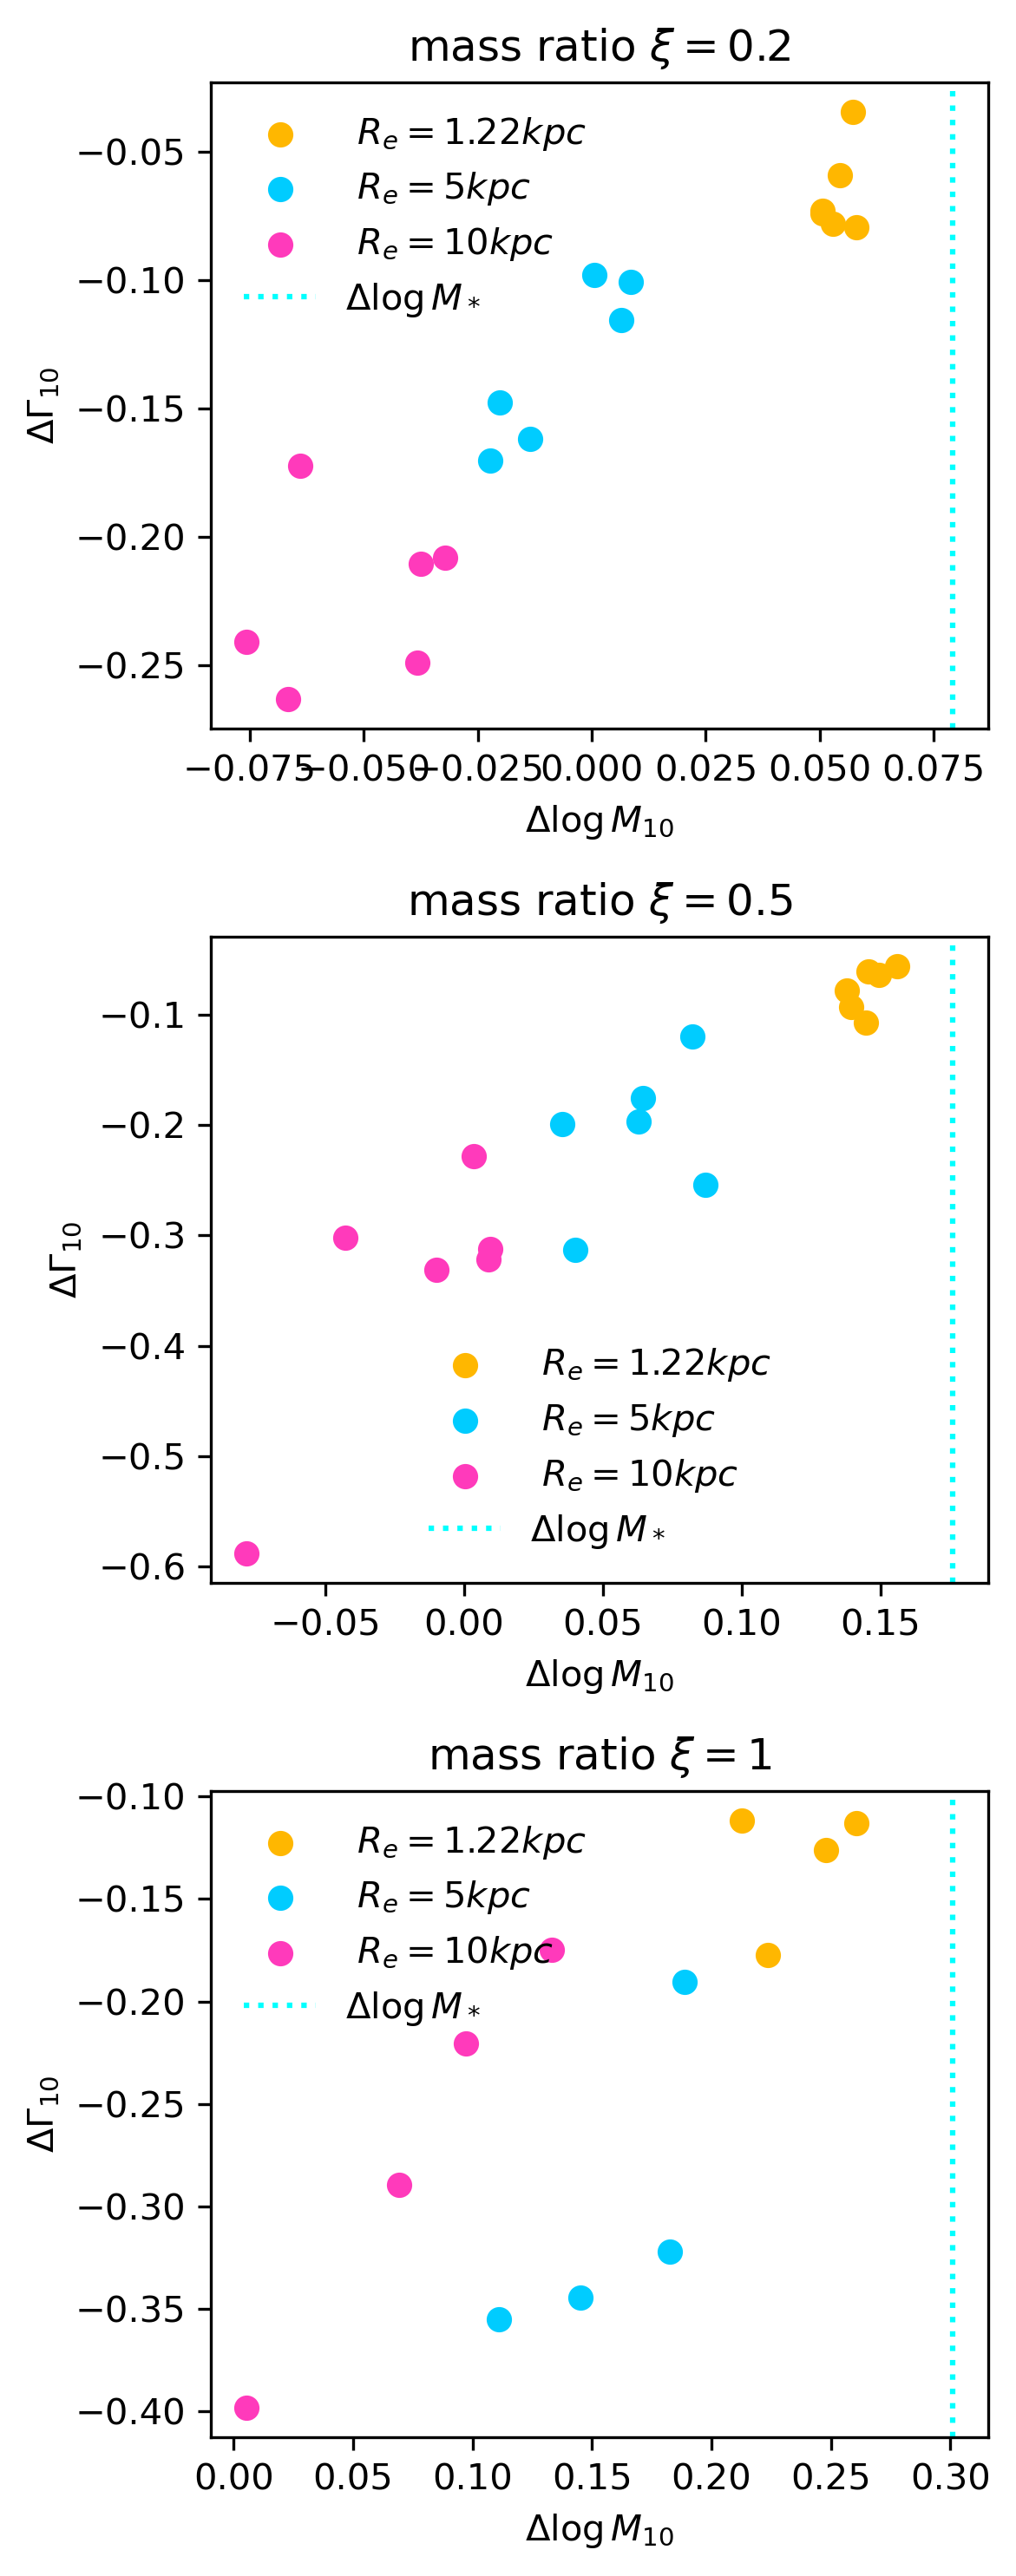
\includegraphics[width=0.75\linewidth]{figure/sim_result.png}
    \caption{ Three panels show the change in $logM_{*,10}$ and $\Gamma_{*,10}$ due to mergers with three different merger ratio $\xi$, while the three colors represent different initial effective radius $R_e$ of the main galaxy.The vertical dotted cyan line shows the logarithmetic change in the total stellar mass for each merger ratio. }
    \label{fig:sim_result}
\end{figure}
% Having done this circulrisation, we are enabled to measure the $M_{*,10}$ and $\Gamma_{*,10}$ of both circularised initial main galaxy and circularised remnant galaxy, and make direct comparison to see how these two quantities grow during the merging process.
\par The next step we should do to generate a mock observation is to give a physical unit to the simulation data. In fact, the unit that \cite{nipoti2009} use in the simulation, for instance, mass,length or velocity, do not have a physical meaning, they are just code units.Only after we specify a physical value for these 'code unit' can we calculate the $M_{*,10}$ and $\Gamma_{*,10}$ for our mock galaxies. We refer such operation as 'rescale' the simulation data. In order to understand what is the impact of mergers on the growth of $M_{*,10}$ and $\Gamma_{*,10}$, we actually need a series of mock galaxies with different initial $M_{*,10}$ and $\Gamma_{*,10}$. Therefore, we need to 'rescale' the simulation data several times to obtain that series of mock galaxies.Traditionally, changing the mass and length unit may affect the timestep used in the simulation, but as we only focus on two snapshots and ignoring the time that one merger event take, we believe this 'rescale' operation would not severely affect our result.If we set the length unit to $1 kpc$, the effective radius of the main galaxy would be $R_e = 1.22 kpc$. We then 'rescale' the simulation data accordingly, generated two additional set of mock galaxies with effective radius $R_e = 7kpc$ and $R_e = 12kpc$.  The reason for choosing these two specific value is explained in detail in Sect.\ref{sec:toy}. We show the evolution in $M_{*,10},\Gamma_{*,10}$ space in Fig.\ref{fig:sim_result}
\par We can easily observe that for all three merger ratios, the parameter $\Gamma_{*,10}$ always shows a decreasing trend, while for larger, more massive galaxies, the decrease in $\Gamma_{*,10}$ tends to be more significant. On the other hand, the growth of parameter $log M_{*,10}$ is a bit more complicated. In general, the growth in $log M_{*,10}$ is always less than the growth in the total stellar mass $\log M_*$, which may indicating that larger fraction of accreted mass are sunk in the outer region of the galaxy. In contrast with the $\Gamma_{*,10}$, smaller galaxies show a larger increase in $log M_{*,10}$. Interestingly, if one pay more attention to the first two panels (top and middle panel), one can find that in some cases, the growth in $log M_{*,10}$ could be even negative after the merger. While for the largest merger ratio $\xi = 1.0$ (bottom panel), the growth in $log M_{*,10}$ is always positive. The negative value informs us that the merger do varies the entire density profile of the galaxy, and the inner region of galaxies may experienced the most significant change comparing with the outer region.The impact on the inner region of galaxies tends to be stronger for mergers with smaller mass ratio.Small mass ratio minor-mergers may flatten the density profile, puffing-up the galaxies hence make $log M_{*,10}$ decrease and $\log M_*$ increase simultaneously.
\subsection{A toy model for the growth of $M_{*,10}$-$\Gamma_{*,10}$ relation due to mergers}
\label{sec:toy}
Firstly, in order to establish a toy model to predict the impact of mergers on the $M_{*,10}$ - $\Gamma_{*,10}$ relation, we need to know how many mass has galaxy grew during a certain period of time, or in other word, during a certain range of redshift. In our work, we adopted the result from \cite{2018moster}, which give a fitting formula of the fraction of stellar mass that accreted onto the main galaxy as a function of redshift for galaxies with different halo mass : 
\begin{equation}
    \label{eq:facc}
    f_{acc}(z) = f_2\exp \left[-f_1(z+1)\right]
\end{equation}
For different halo mass, the parameter $f_1$ and $f_2$ are different, as shown in table~\ref{tab:facc}. Here we only show the fitting parameter for two different, relatively large halo mass, as we only focus on the massive quiescent galaxies in our observation sample.
\par The next step is to estimate the stellar mass given the halo mass, hence we need the stellar-to-halo mass relation (SHM relation). This relation has a relatively large scatter, therefore inferring average halo mass from a given stellar mass is not equivalent to inferring the stellar mass from a given halo mass. In this work, we aim to know the average fraction of accreted mass, hence we need know what stellar mass correspond to a average halo mass $10^{13}M_\odot$ (or $10^{14}M_\odot$).  We thus use Fig.4 in \cite{2020moster} to operate a rough estimate on the stellar mass. For $M_h = 10^{13}M_\odot$, the stellar mass is about $10^{11.1}M_\odot$, while for $M_h = 10^{14}M_\odot$, the stellar mass is about $10^{11.7}M_\odot$.We then make narrow stellar mass bins in our final sample, then calculated the median value of $M_{*,10}$ : $10^{10.9}M_\odot$ and $10^{11.4}M_\odot$ respectively.
\par Having estimate the $M_{*,10}$, we start from the $\Gamma_{*,10}$ - $M_{*,10}$ relation of the highest redshift bin ($0.34 < z \leq 0.4$ ) to estimate the $\Gamma_{*,10}$ for these two stellar mass. Then we try to 'rescale' our simulation data to let the 'rescaled' mock galaxy have a $\Gamma_{*,10}$ that is close to the estimated value.  The 'rescaled' mock galaxy correspond to halo mass $M_h = 10^{13}M_\odot$ has a effective radius $R_e = 7 kpc$ with $\Gamma_{*,10} \approx 1.57$, while another mock galaxy has $R_e = 12kpc$ with $\Gamma_{*,10} \approx 1.39$.These are the initial state of mock galaxies. We hope to explain the change of the $M_{*,10}$ - $\Gamma_{*,10}$ relation from the highest redshift bin to the lowest redshift bin using our toy model, hence we calculated the mass that has accreted to the galaxy during that range of redshift using Eq.\ref{eq:facc} and then translate the accreted mass fraction to the numbers of merger events with different merger ratio ($\xi = 1.0,0.5,0.2$). 
 $\Delta M_{*,10}^{\text{total}}$ and $\Delta \Gamma_{*,10}^{\text{total}}$ due to an entire merger event is already obtained and is shown in Fig.\ref{fig:sim_result}, we thus estimate the growth of $M_{*,10}$ and $\Gamma_{*,10}$ by multiplying the number of mergers with the $\Delta M_{*,10}^{\text{total}}$ and $\Delta \Gamma_{*,10}^{\text{total}}$.In brief, we assume the initial mock galaxies have experienced only one type of merger during the redshift interval and calculated the possible growth in $M_{*,10}-\Gamma_{*,10}$ space. Adding the growth to the initial state, we thus obtain the final state of our mock galaxies. 
The result is shown in Fig.\ref{fig:toy}.The blue points shows the initial $M_{*,10}$ and $\Gamma_{*,10}$, and the other points shows the final state of these two mock galaxies due to different types of merger. In comparison, we also plotted the $M_{*,10} - \Gamma_{*,10}$ relation in the lowest redshift bin in pink line. 
\par From Fig.\ref{fig:toy}, we could conclude that mergers would always change the slope of the $\Gamma_{*,10} - M_{*,10}$ relation, resulting in a steeper relation. The lower the merger mass ratio, the more significant the change in slope. In addition, mergers would also induce a normalization change in the $\Gamma_{*,10} - M_{*,10}$ relation. The three result lines are all lays below the initial state. The change in normalization also have a similar trend as the change in slope, the lower merger mass ratio would induce a more intense decrease in normalization. 
\par Having predicted the impact of different mergers on the $\Gamma_{*,10} - M_{*,10}$ relation, we then compare the result with our observation sample. Recalling that we calculated the possible number of merger events from $z \approx 0.37$ to $z \approx 0.17$ in order to make comparisons with the lowest redshift bin in our observation sample, we thus add the $\Gamma_{*,10} -M_{*,10}$ relation in redshift bin $0.15 < z \leq 0.21$ in Fig.\ref{fig:toy} in pink line. It's easy to observe that this pink line has a steeper slope comparing with the blue one. In fact, the slope of the pink line is more steeper than all the other lines in this figure, even for the orange dotted line which represent the predicted $\Gamma_{*,10} - M_{*,10}$ relation due to the merger with the lowest mass ratio $\xi = 0.2$. In the context of merger, we could reach a qualitatively conclusion that this steep slope indicate the growth of $M_{*,10}$ and $\Gamma_{*,10}$ is induced by mergers with smaller mass ratio, for instance, $\xi = 0.1$. However, the pink line is all have a larger normalization than the three predicted line. It is apparent that none of the predicted line is in agreement with that pink one. Therefore, we need to be careful to interpret the result in Fig.\ref{fig:toy}, as this disagreement may come from from various systematic.
% It is easy to observe that the change in slope of the $M_{*,10} - \Gamma_{*,10}$ becomes more significant for lower merger mass ratio. However, even for the lowest merger mass ratio $\xi = 0.2$, the slope of the $M_{*,10} - \Gamma_{*,10}$ relation of the final state is still less steep than the relation in the lowest redshift bin. On the other hand, the normalization of the $M_{*,10} - \Gamma_{*,10}$ relation of three merger ratio all deviated from that in lowest redshift bin. In fact, we suspect the $M_{*,10}$ in the highest redshift bin might be underestimate, hence the difference in normalization might be smaller than shown in Fig.\ref{fig:toy}.
\begin{figure}
    \centering
    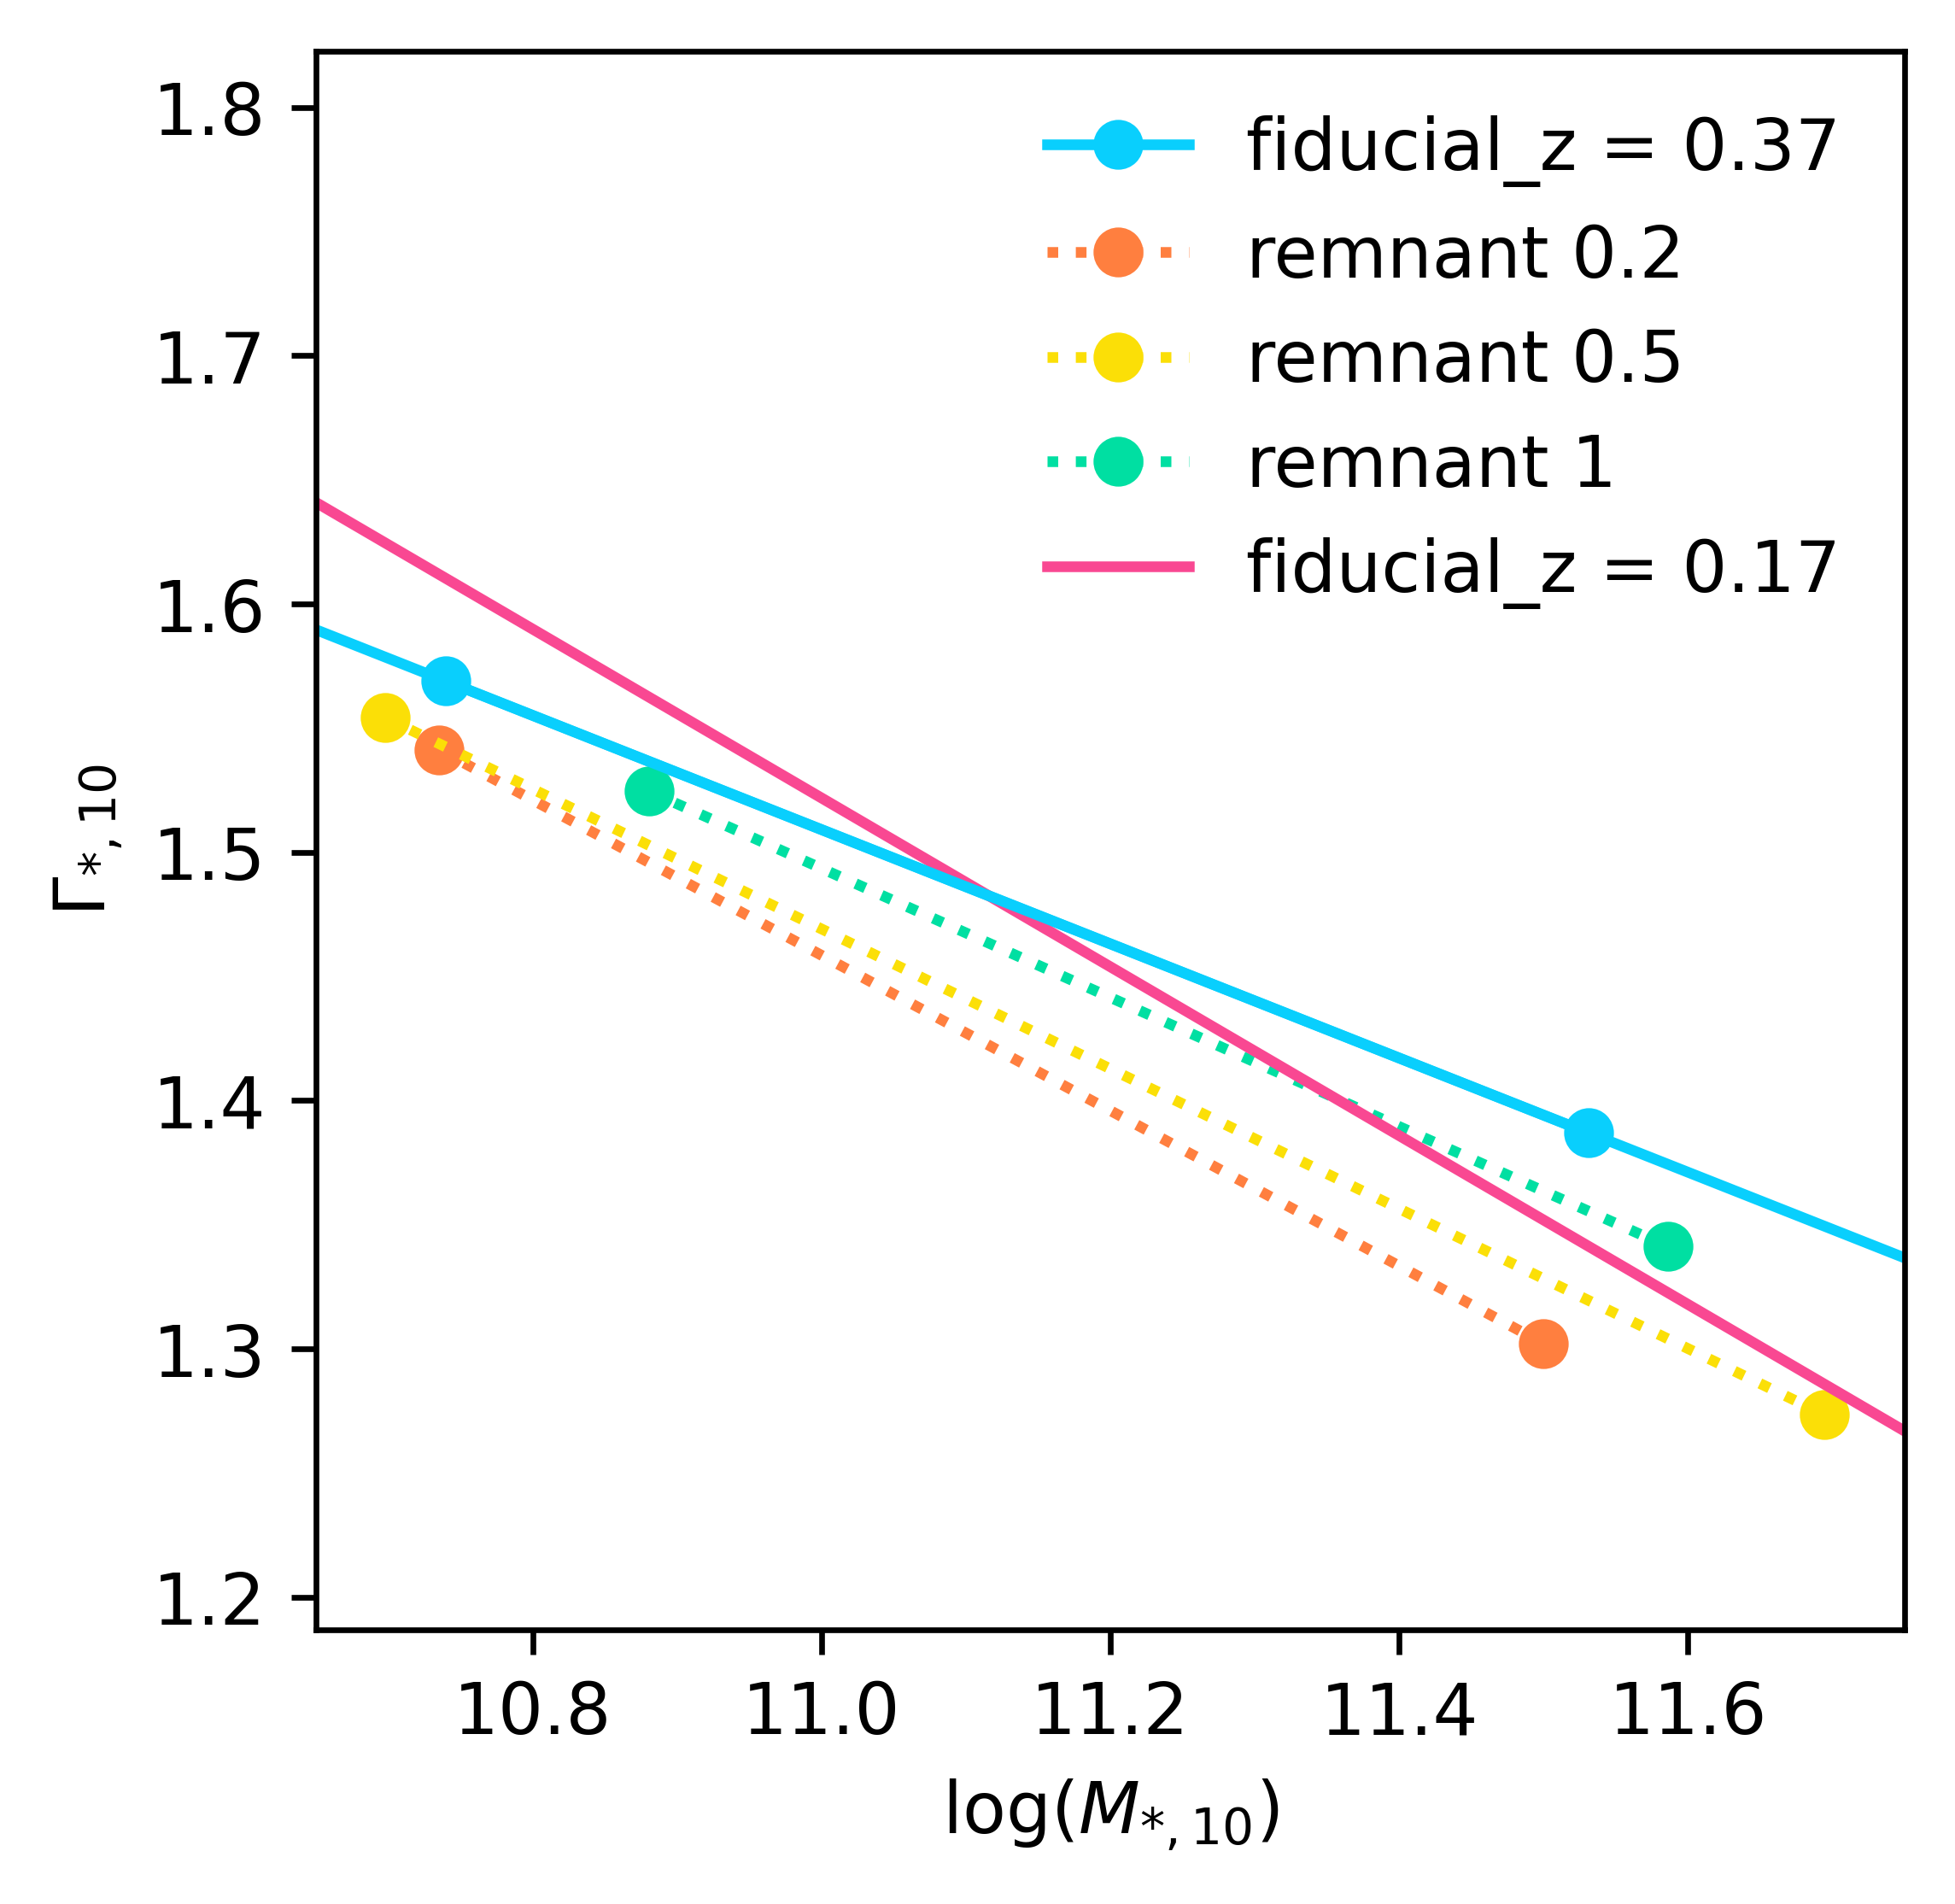
\includegraphics[width=0.8\linewidth]{figure/toy_model.png}
    \caption{The growth of $M_{*,10}$ and $\Gamma_{*,10}$ due to mergers in our toy model. The blue and red points represent the growth of $M_{*,10}$ and $\Gamma_{*,10}$ respectively. The error bar represents the standard error in each bins.}
    \label{fig:toy}
\end{figure}
\begin{table}
    \centering
    \caption{Simulation parameters for different sets of simulation. }
    \label{tab:facc}
    \begin{tabular}{ccc}
        \hline
        % \hline
        $\log M_h$ & $f_1$ & $f_2$  \\
        \hline
        13& 1.09 & 0.55  \\
        14 & 0.94 & 1.43  \\
        
        \hline
    \end{tabular}
\end{table}
% \section{Result}
% \subsection{The growth of $M_{*,10}$ and $\Gamma_{*,10}$ in simulation}
% \par In practice, if we want to understand what is the impact of mergers on the growth of $M_{*,10}$ and $\Gamma_{*,10}$, we actually need a series of mock galaxies with different initial $M_{*,10}$ and $\Gamma_{*,10}$. 
% Fortunately, the mass,length, time and velocity in the simulation that we utilized are not in physical unit, but in code unit. That means we have the freedom to 'rescale' the simulation data, i.e. specify a physical value for these 'code unit', to generate galaxies with different size and mass. Traditionally, changing the mass and length unit may affect the timestep used in the simulation, but as we only focus on two snapshots and ignoring the time that one merger event take, we believe this 'rescale' operation would not severely affect our result. The default scale of the simulation set the length unit to $1 kpc$ so that the effective radius of which is $R_e = 1.22 kpc$. We then make two other modification to make the initial main galaxy has $R_e = 5,10 kpc$, meaning that the physical value of one code length unit is $4.1, 8.2 kpc$ respectively in each modification.Therefore, for each set of simulations, we have three pairs of main and remnant galaxies. We then measured the $M_{*,10}$ and $\Gamma_{*,10}$ of all six galaxies in one set for all sets of simulations. The result is shown in Fig.\ref{fig:sim_result}. 



% \subsection{Observation result}
% \label{sec:obres}
% \par Having investigate the result in simulations, we then operate the measurement to our observation sample. As a consequence of the completeness cut, galaxies with lower $M_{*,10}$ value at higher redshift would be absent in our sample. To investigate the evolution trend in $M_{*,10 } - \Gamma_{*,10}$ relation, we have to either narrow the redshift range to include more low-$M_{*,10}$ galaxies or narrow the $M_{*,10}$ range to include more high-redshift galaxies. In this work, we choose the latter one, meaning that we only focus on massive quiescent galaxies whose $M_{*,10} \geq 10^{10.9} M_{\odot}$. In addition, we set a lower limit on the redshift range $ z \geq 0.15$. It's easy to observe some vertical stripe-like feature in Fig.\ref{fig:completeness_cut} at low redshift end, and is thought to be the effect of large scale structure by \cite{GAMAmain}. It is reasonable as the comoving volume at low redshift is relatively smaller, so it is more likely to suffer from cosmic variance. We thus determined this low-redshift cut in order to avoid such cosmic variance. The final sample we used to investigate the evolution is show by cyan dots in Fig.\ref{fig:completeness_cut}. We binned the sample in redshift and $M_{*,10}$, then calculated the median value of $\Gamma_{*,10}$ in each bin. The $\Gamma_{*,10}$ result is shown as a function of $M_{*,10}$ in Fig.\ref{fig:mg_relation} and as a function of redshift in Fig.\ref{fig:gamma}.

% \begin{figure}
%     \centering
%     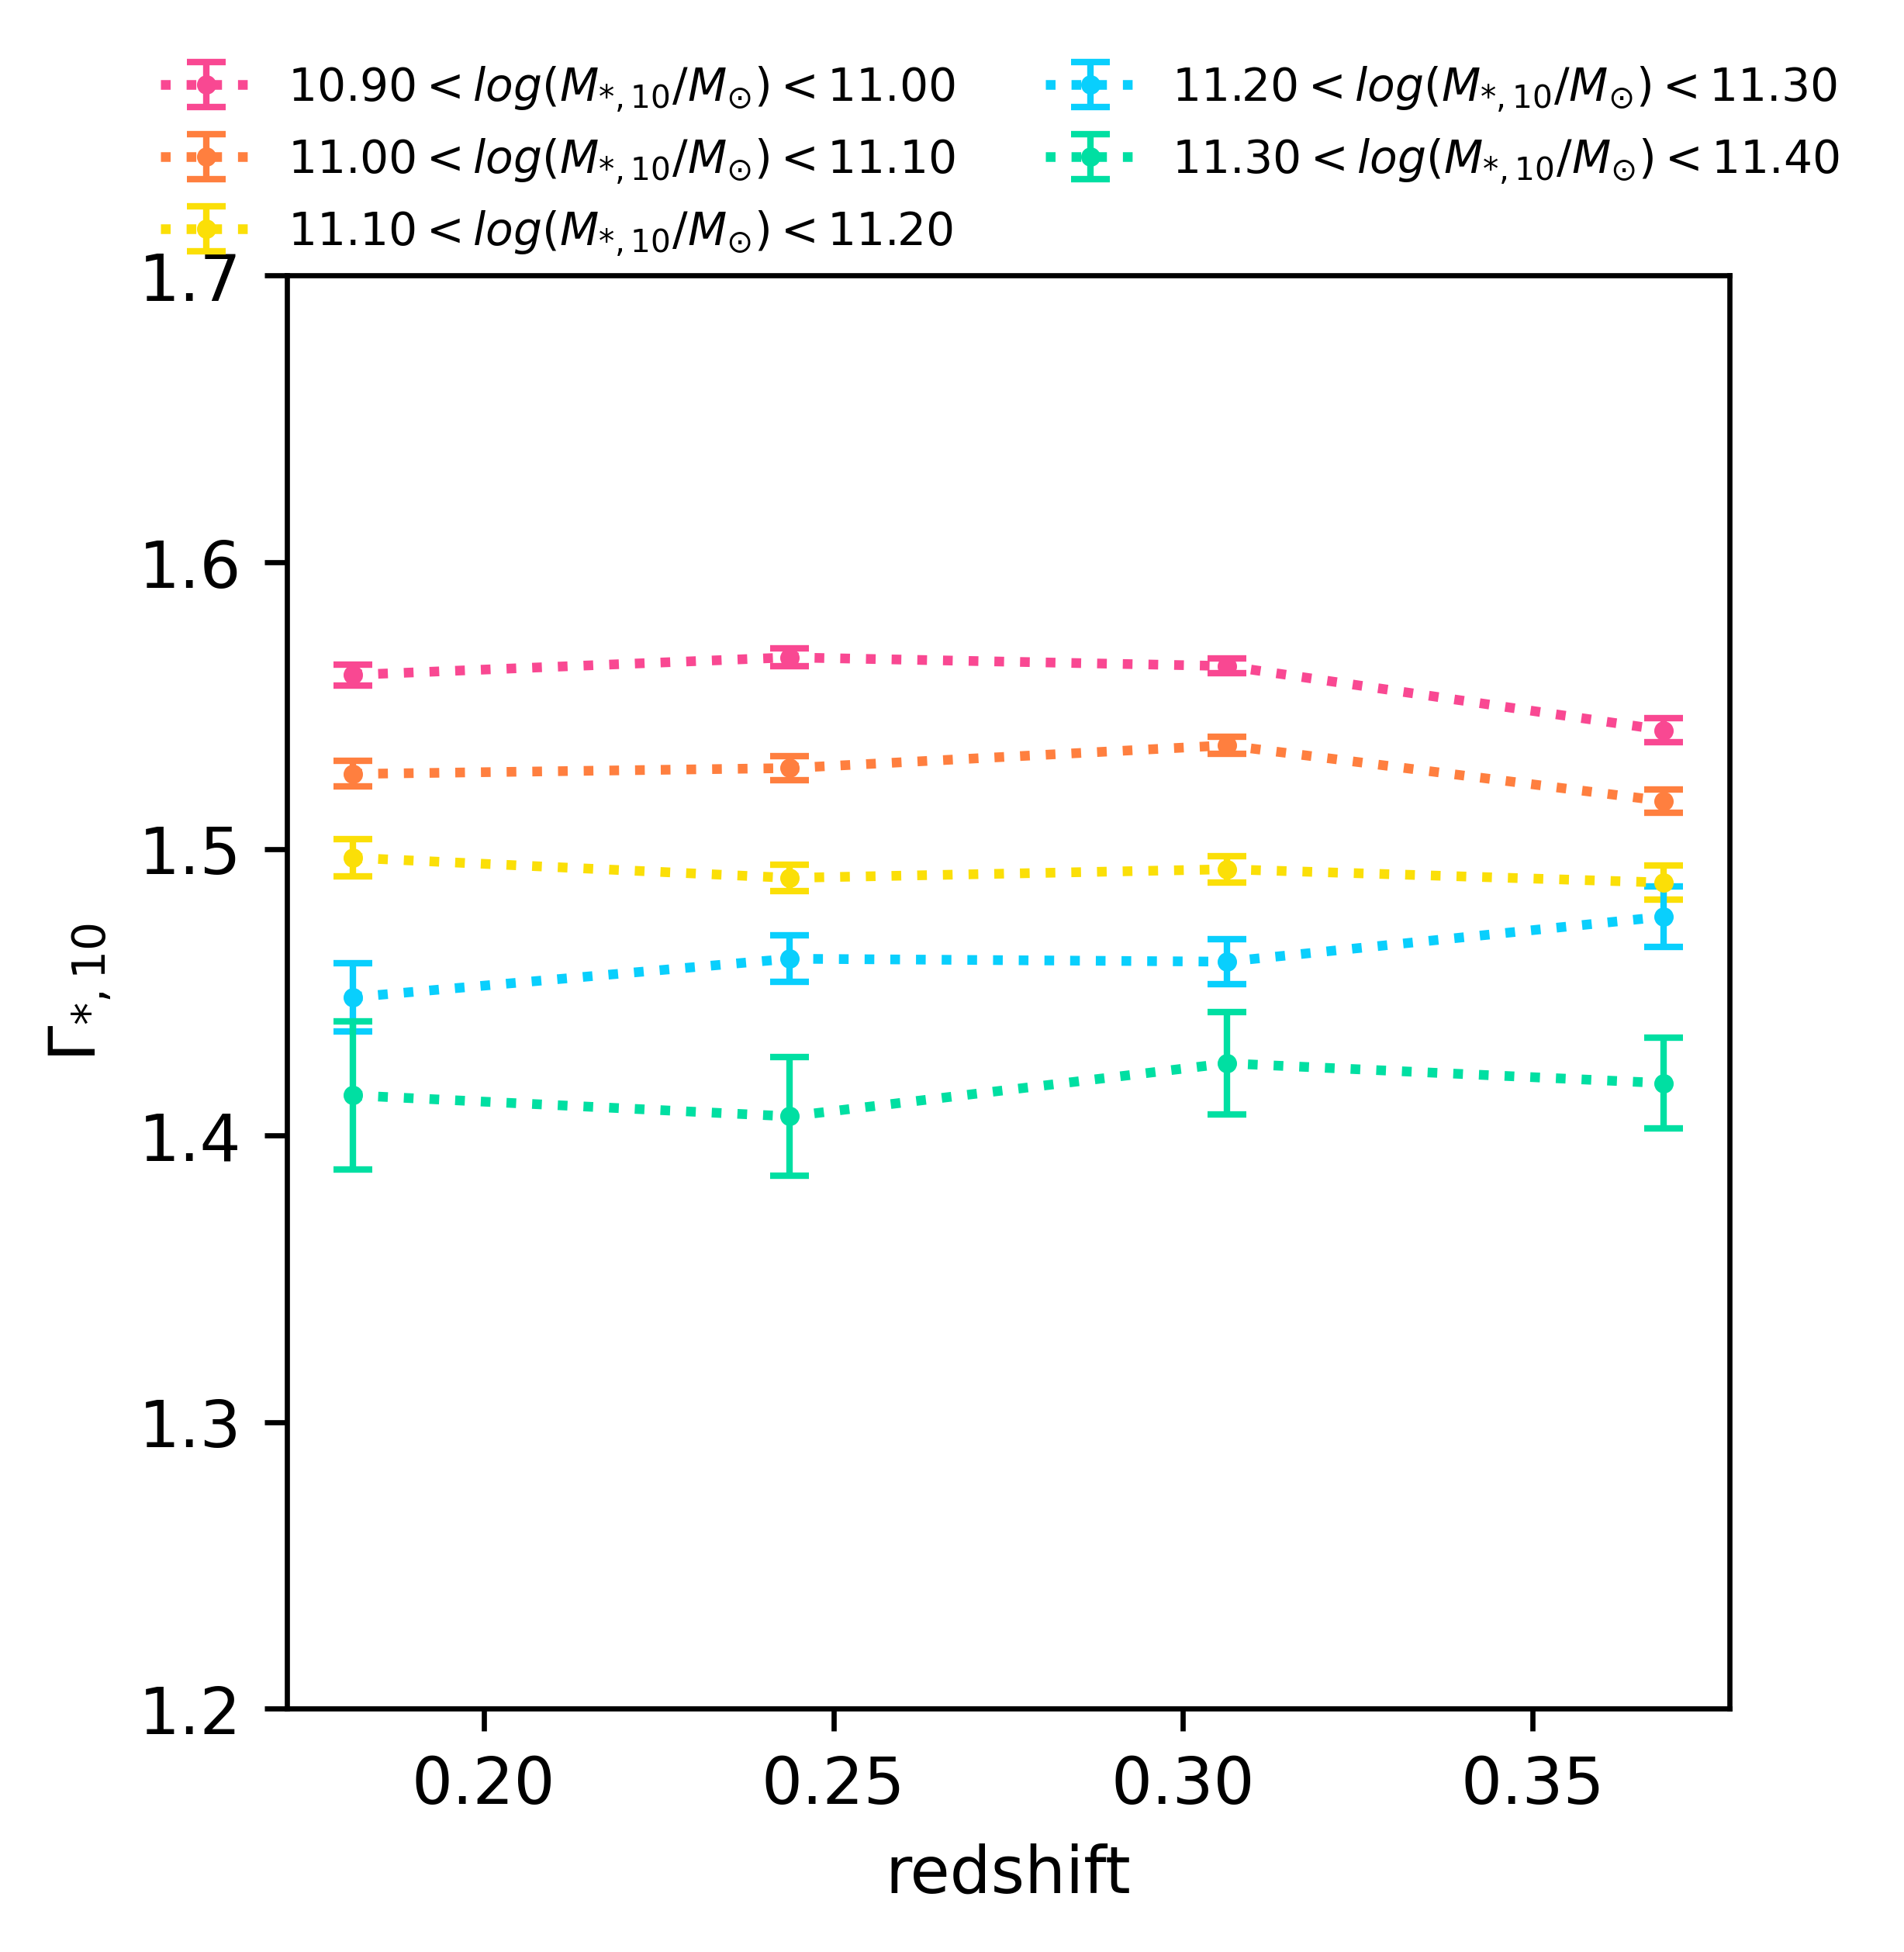
\includegraphics[width=\linewidth]{figure/gamma.png}
%     \caption{$\Gamma_{*,10}$ as a function of redshift in each $M_{*,10} $ bin. The sample are divided into five different $M_{*,10}$ bins.The error bar represents the standard error in each bins.}
%     \label{fig:gamma}
% \end{figure}
% \par In Fig.\ref{fig:mg_relation}, we could observe a anti-correlation between $M_{*,10}$ and $\Gamma_{*,10}$. Comparing the data in four redshift bins simultaneously, we can hardly see the evolution trend in this relation. In addition, if we focus on $\Gamma_{*,10}$ only, as shown in Fig.\ref{fig:gamma}, we could reach a similar conclusion that there is no significant evolution in $\Gamma_{*,10}$.The $\Gamma_{*,10}$ value in five different $M_{*,10}$ are all almost constant as the redshift grows. The error bars in these two plots are standard error in each bin, i.e the standard deviation divided by the square root of the number of galaxies in each bins. The error bar is relatively larger at higher $M_{*,10}$ end, but it does not affect our conclusion as in Fig \ref{fig:mg_relation}, the data points are still overlapping with each other in the same $M_{*,10}$ bin and the $\Gamma_{*,10} - z$ relation can still be reckoned as a horizontal line. 
% \par From the observation result shown in Fig.\ref{fig:mg_relation} and Fig.\ref{fig:gamma}, we can hardly observe any evolution trend in $M_{*,10} - \Gamma_{*,10}$ relation during the redshift range $ 0.15 \leq z \leq 0.4$ . However, using observation data alone does not enable us to reach the conclusion that galaxies do not evolve at that period of time, cause various evolution scenarios may result in the lack of growth in $M_{*,10} - \Gamma_{*,10}$ relation. For instance, if galaxy evolves along the $M_{*,10} - \Gamma_{*,10}$ relation shown in Fig.\ref{fig:mg_relation}, then this relation would not shows any growth in its intercept or slope and thus mimic the evolution trend. Nevertheless, taking the advantage of binary merger simulations, we are informed that how the $M_{*,10} $ and $\Gamma_{*,10}$ would evolve if the galaxies do experience mergers. The fact is, no matter what kind of merger one galaxy may experience, it would always leave a observable impact on the $M_{*,10} - \Gamma_{*,10}$ relation. We may consider a idealized condition that every galaxy experienced a merger during the redshift interval $0.4 \geq z \geq 0.15$ with mass ratio $\xi = 0.2$. From the upper panel of Fig.\ref{fig:sim_result} we can observe that this kind of merger will make massive galaxies goes down more rapid in $M_{*,10}-\Gamma_{*,10}$ diagram than the less massive ones, which will drive this relation to be steeper. In addition, merger will increase $M_{*,10}$ of less massive galaxies while decrease $M_{*,10}$ of more massive ones, and thus twist the $M_{*,10}-\Gamma_{*,10}$ relation in a clockwise direction, i.e. steeper the slope more intensively. However, we could not observe any evidence of such evolution trend in our observation sample. As is shown in Fig.\ref{fig:mg_relation}, the slope of such relation in four different redshift bins can be considered as nearly identical. Therefore, we make our conclusion that galaxies do not experience significant growth due to mergers in the redshift range $0.15 \leq z \leq 0.4$.
\section{Discussion}
\label{sec:4}
\subsection{Effect of spiral arms}
The goal of our work is to investigate the evolution of quiescent galaxies without requiring the total flux of one galaxy. We expect all our galaxies can be perfectly described by a single S\'{e}rsic surface brightness profile, i.e. all galaxies are elliptical in shape. However, in reality, we only make a selection criteria based on the star-forming activities which is inferred from index $Dn4000$, hence we cannot exclude the potential risk of the contamination from spiral galaxies. Therefore, we need to know how spiral arms would affect the measurement of $M_{*,10}$ and $\Gamma_{*,10}$.
\par  \cite{Ale22_spiral} performed a detailed analysis on the effect of spiral arms on the measurement of both total flux and the half-light radius $R_e$. Generally speaking, the existence of spiral arms would generate a bump in surface brightness near the light-weighted radius of the spiral arm. According to Fig.6 of \cite{Ale22_spiral}, the best-fitting S\'{e}rsic model would begin to show a significant deviation from the real data at larger radii in respect to that "bump", while the inner region is not affected. This deviation would thus result in the bias in both total flux and $R_e$. In particular, the bias that introduced by spiral arm have a dependence on the ratio between the light-weight radius of spiral arm and the half-light radius of the galaxy. Both bias in total flux and $R_e$ shows a increasing trend as this ratio grows while the ratio is smaller than about $1.8$ and then decrease slightly as the ratio grows further, according to Fig.7 in \cite{Ale22_spiral}.
\par In fact, one of the reason that we choose $10kpc$ as the fixed aperture is that this physical size is close to the average half-light radius of massive quiescent galaxies. Therefore, we can qualitatively conclude that the spiral arm of galaxies with similar size and mass of our sample will not leave a significant bias in our measurement. In one hand, if the spiral arm do affect the total flux and $R_e$ significantly, then the light-weight radius of spiral arm has to be significantly larger than the half-light radius.However, the large size of the spiral arm also means the bump in surface brightness profile occurs at larger radii in respect to $10kpc$, making the $10kpc$ as the unaffected inner region. On the other hand, if the aperture $10kpc$ cannot be considered as the unaffected inner region, i.e. the light-weight radius of spiral arm is close to the half-light radius, then the total bias that introduce by spiral arm would be small, no matter the bias in $M_{*,10}$ or $\Gamma_{*,10}$.
\par Although we believe that out work is not significantly biased by spiral arm, one still need to be careful when dealing with samples with smaller size. For instance, if the $R_e \approx 5kpc$, i.e. $1.8 \times R_e \approx 10kpc$,then the bias introduced by spiral arm will become significant, as the bias reaches its maximum while the bump also close to the $10kpc$ aperture where we focus on. In this case, we may suggest to use a smaller aperture, for instance $5kpc$, to avoid the bias.  
\subsection{Limitations of our method}
In this work, we adopted a new method that only focusing inside a fixed aperture $10kpc$, instead of attempting to obtain the entire light. Unlike the traditional parameter: effective radius $R_e$ which is sensitive to different approaches of modeling the surface brightness profile, the fixed aperture in our method do not have such dependence. Therefore, we believe that our method provides a more robust way to make comparisons between simulations and observations and among different observations. 
\par However, this robustness on the aperture size in turn placed a limitation on the sample selection. To ensure the aperture measurement is accurate, we need to obtain the spectrum of galaxies for a precise spectroscopic redshift measurement. Actually, our work is not affected by this requirement, as we also need the spectroscopic data to distinguish the quiescent galaxies from its star-forming counterparts. If we want to apply this method to a population of galaxies that do not rely on spectroscopic data to be selected , for instance, early type galaxies, then this spectroscopic data requirement would limit our sample to a relatively smaller range in both redshift and stellar mass. The work of  \cite{KiDs_Roy} could be a good example. They also use KiDs data, which is similar to ours, to investigate the evolution on the scaling relation of both early-type and late-type galaxies. Without the requirement of spectroscopic data, they use photometric redshift hence the sample could extend to higher redshift $z \approx 0.6$ and lower total stellar mass $M_* \approx 10^{11} M_{\odot}$ comparing to our sample, under the condition that they use KiDs DR2 data which has a significant smaller sample size than DR4.
\par To overcome this limitation, one may consider to use such surveys which cover a small field in the sky but could go to a deeper magnitude. For instance, using HSC \citep{HSC16} images combining with spectroscopic data from SHELS F2 \citep{Geller14} as \cite{damjanov2019} did. SHELS F2 could reach $95\%$ complete down to r-band magnitude $r = 20.6$ in $3.98~deg^2$ area, roughly one magnitude deeper and covers about 55 times smaller region than GAMA. Nevertheless, the sample used in \cite{damjanov2019} can still reach lower stellar mass limit $M_* \approx 10^{10} M_{\odot}$. However, the shortcoming of choosing deep and narrow field survey is that the sample size would be relatively small, which limit the precision of the measurement. In addition, the small field would also make the sample more sensitive to the cosmic variance.
If one want to further analyse the number density of his sample, using such survey would be a bad choice. Hopefully, the incoming stage-IV survey could widen the survey coverage while deepen the survey limiting magnitude. We then thus do not need to make compromise between the coverage and the depth of the survey.  
% \subsection{Number density of quiescent galaxies}
% In fact, to infer the growth mechanism that quiescent galaxies may undergo, the number density could provide some valuable information in addition to the evolution trend of $M_{*,10} - \Gamma_{*,10}$ relation alone. For instance, \cite{van_dokkum_growth_2010} select galaxies with constant number density through different redshift bins, in order to select the same population of galaxies and therefore attained the growth of such population. Recently,
%  \cite{Bundy2017} has studied the evolution in the number density of massive quiescent galaxies. Having considered a number of systematic that may affect the number densities, they claimed they did not detected a significant growth for these massive quiescent galaxies. 
% \par However, the most important thing in studying the number density is exactly the systematics. As the number of massive galaxies becomes less and less in high mass end, the number density becomes more and more sensitive to some potential systematics. Actually, as the narrow redshift and $M_{*,10}$ range that we are focusing, our expectation is that the number density would not change significantly during this period of time. In order to reach the conclusion that the number density of massive quiescent galaxies stays constant during $0.15 \leq z \leq 0.4$, we need to be more careful about the systematics. To eliminate these systematic biases, we need to perform some detailed analysis on stellar mass estimation, the cosmic variance, for instance. Therefore, we leave the investigation on number density of massive quiescent galaxies in our sample to the future work.  
\subsection{Possible systematic in stellar mass estimate}
This concern arise from the prediction of our toy model. In Fig.\ref{fig:toy}, we could observe that although the slope of the $\Gamma_{*,10} - M_{*,10}$ relation in the lowest redshift bin, which is shown in pink line, is already close to the predicted $\Gamma_{*,10} - M_{*,10}$ relation, especially for the orange line which represent the predicted relation due to the merger with the lowest mass ratio $\xi = 0.2$, the pink line still lay above the orange line. One possible solution to this discrepancy is that the stellar mass in the highest redshift bin is underesitmated, as this discrepency can be easily reduced by moving the blue line and the three predicted lines rightward. 
\par  In fact, we also observed a similar discrepancy in the number density of quiescent galaxies. The number density are shown in Fig.\ref{fig:number_density}. The blue line represent the number density in the highest redshift bin, and it also seems to be lower than the other three. However, if we assume a 0.1dex bias in stellar mass estimate, and thus correct this bias by simply moving the blue line rightward for the same amplitude, we could observe that the corrected number density are in a good agreement with the other three redshift bins. Similarly, if we apply a same correction in Fig.\ref{fig:toy}, we could also observe the pink line agrees better to the orange line, although it is not a perfect agreement as we have pointed out in Sect.\ref{sec:toy} that the true mechanism should be mergers with less mass ratio.
\par However, all these above is just a crude guess on the systemic in stellar mass estimate. In fact, we could not just make the assumption that the number density stays constant during $0.15 \leq z \leq 0.4$. The evolution in number density is also informative, it could provide valuable information in addition to the evolution trend of $M_{*,10} - \Gamma_{*,10}$ relation alone. For instance, \cite{van_dokkum_growth_2010} select galaxies with constant number density through different redshift bins, in order to select the same population of galaxies and therefore attained the growth of such population; \cite{Bundy2017} has studied the evolution in the number density of massive quiescent galaxies. Having considered a number of systematic that may affect the number densities, they claimed they did not detected a significant growth for these massive quiescent galaxies. Therefore, if we assume the number density of quiescent does not evolve, that would indicate the galaxies itself do not grow, which are in tenstion with our previous conclusion. However, if we want to further analyse the number density of our sample, we have to make detailed analyse on the stellar mass estimate of our sample to overcome the potential bias, such as a underestimation of stellar mass. At current stage, we lack a quantitively analyse on how much has the stellar mass estimate being biased, hence our ability to obtain information from the number density and the normalization of $\Gamma_{*,10} - M_{*,10}$ relation is limited. Nevertheless, we believe the slope of such relation can still teach us something about the growth mechanism of quiescent galaxies.  
\begin{figure}
    \centering
    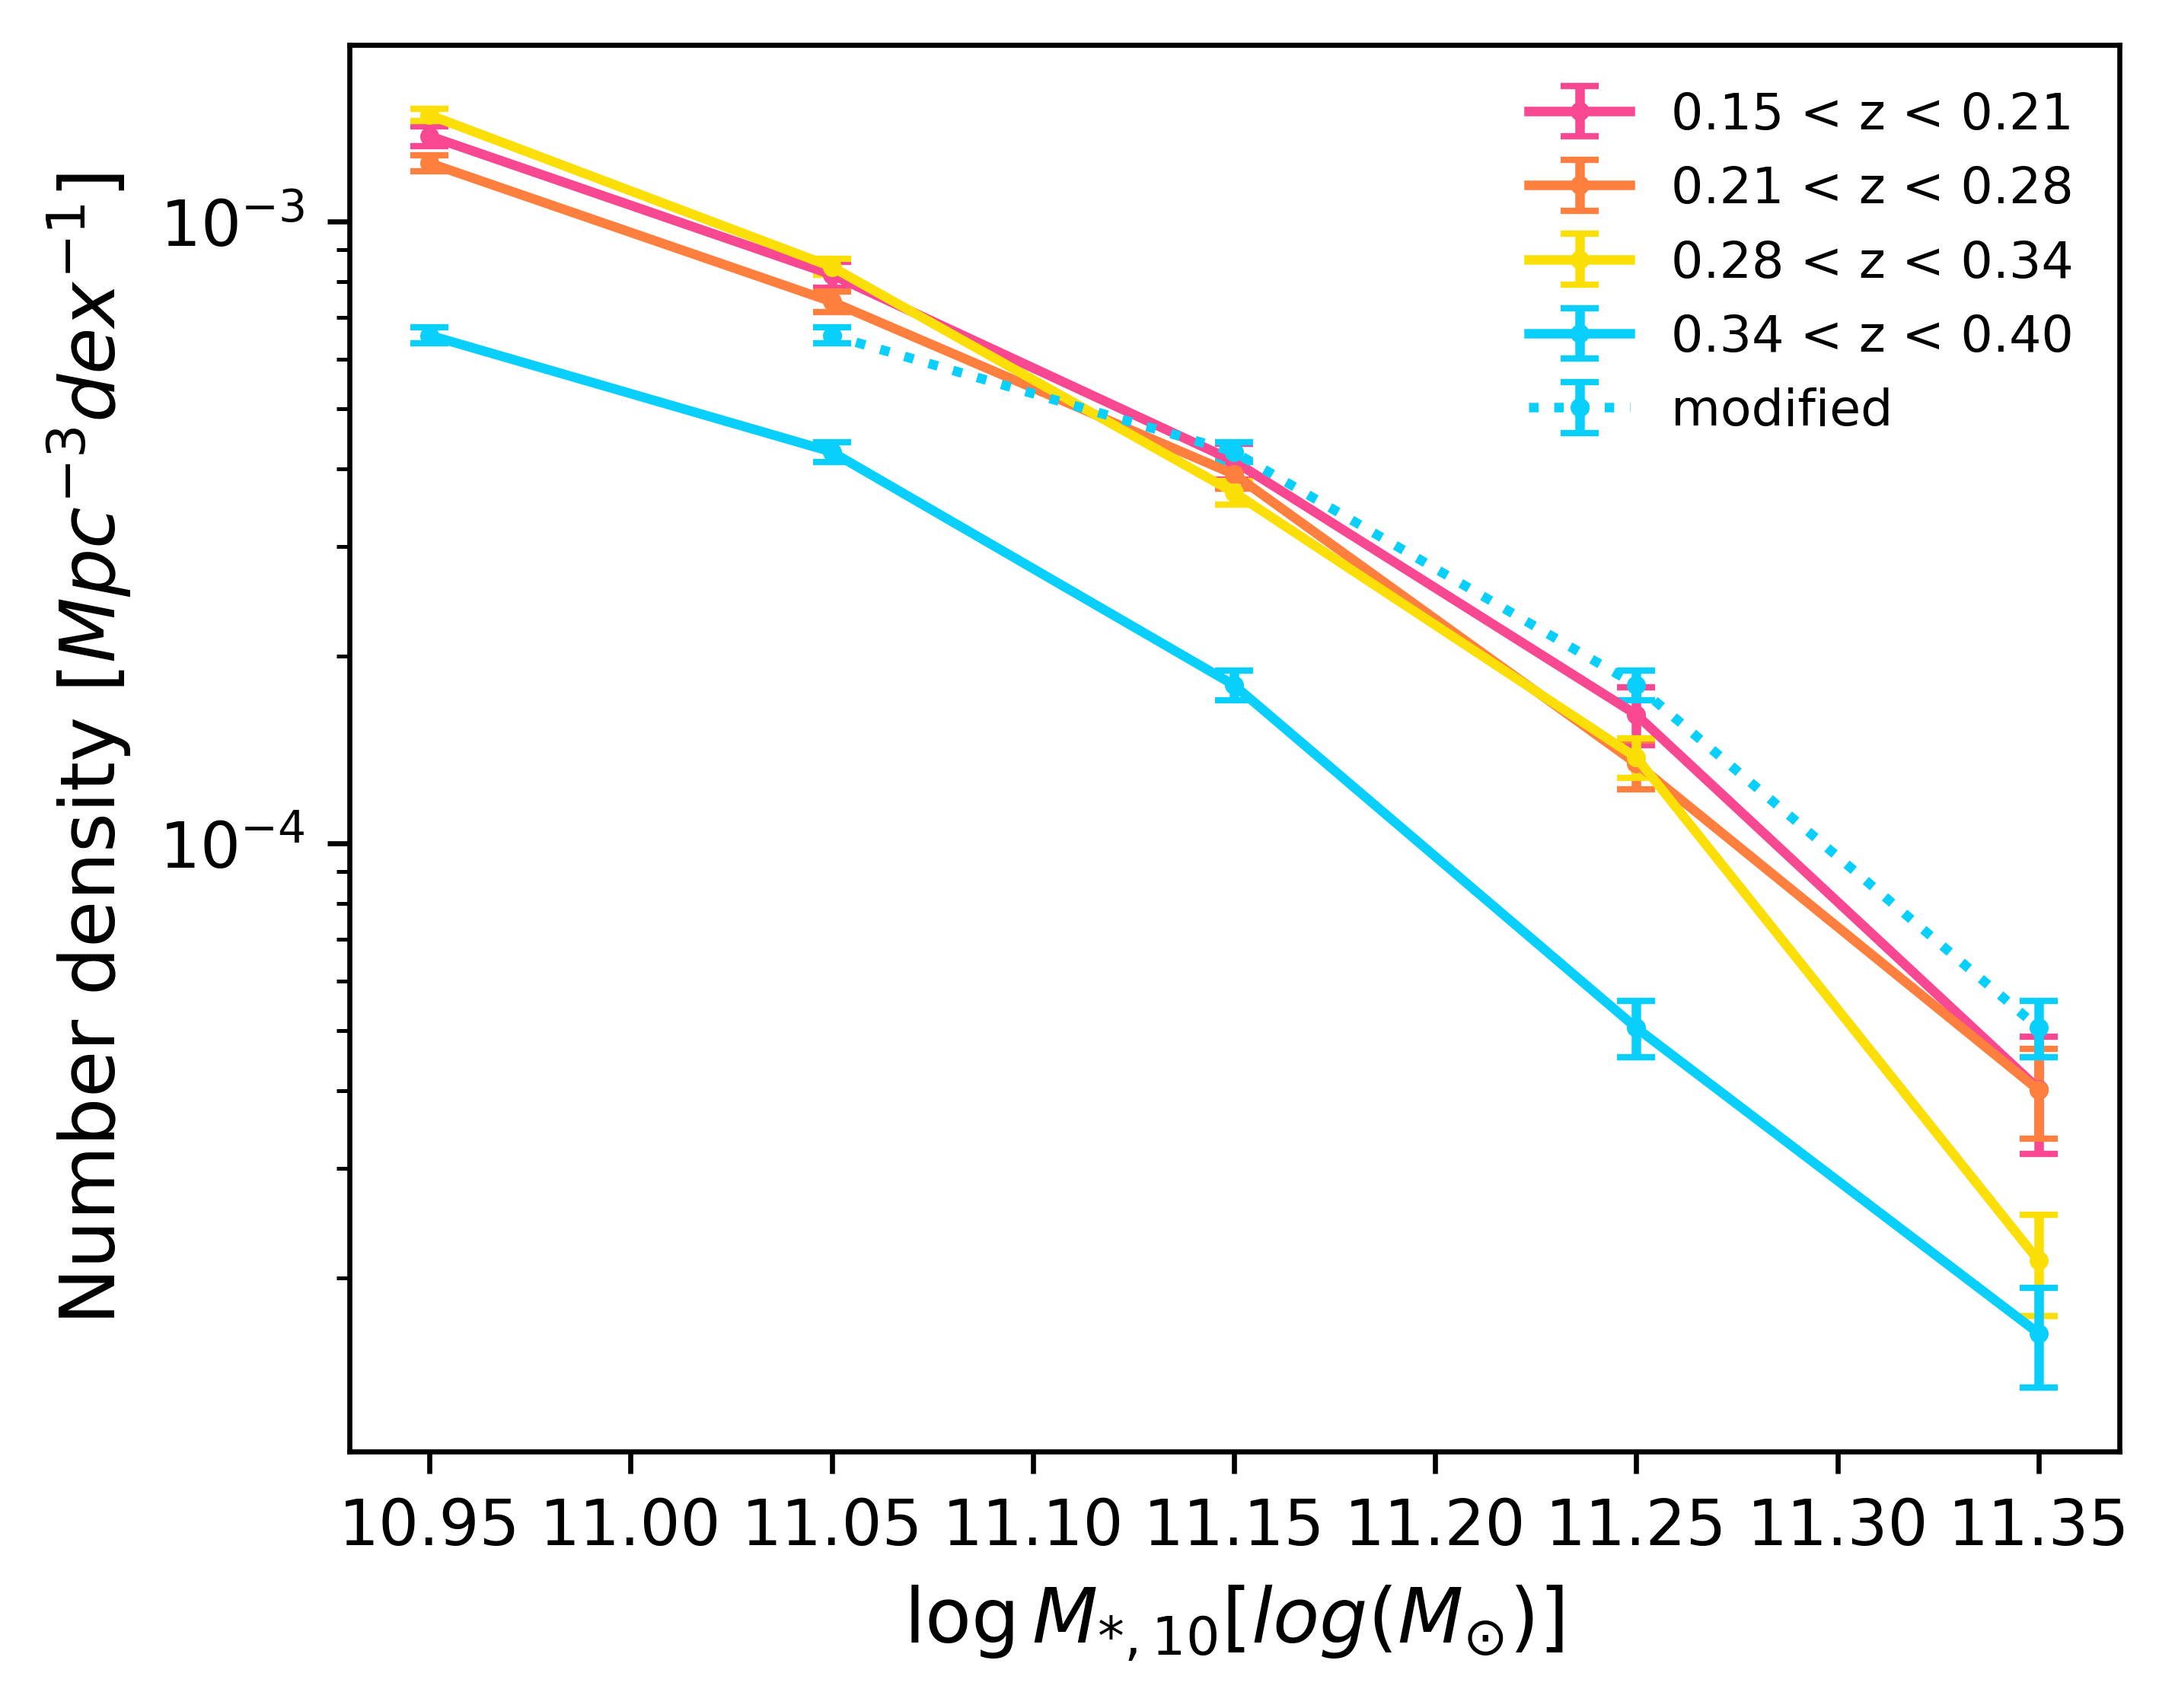
\includegraphics[width=0.95\linewidth]{figure/number_density.png}
    \caption{The number density of quiescent galaxies in each redshift bins in our sample. We also move the blue solid line rightward for 0.1dex to illustrate the underestimation of the stellar mass, and is shown in dotted blue line.We can observe that the corrected number density are in a good agreement with the other three redshift bins, which indicate a possible 0.1dex bias in stellar mass estimate.}
    \label{fig:number_density}
\end{figure}
\section{Conclusion}
\label{sec:5}
In our work, we provide a new perspective to investigate the evolution of quiescent galaxies. Instead of trying to obtain the information of stellar mass and gravitational radius from the entire light of one galaxy, we switch our attention into the inner region. In particular, we focus on a fixed physical aperture $10kpc$ and measure the mass and mass-weighted projected surface brightness slope $\Gamma_{*,10}$ within. Although some information of the outer region is artificially ignored, these new parameterization could still provide us sufficient information to investigate the evolution of quiescent galaxies.
\par First, combining KiDs imaging with GAMA spectroscopy, we measured the $\Gamma_{*,10} - M_{*,10}$ relation in four different redshift bins and corrected for the Eddington bias. The result is shown in Fig.\ref{fig:mg_relation}. We observed the highest redshift bin has a steeper slope in the $\Gamma_{*,10} - M_{*,10}$ relation than the other three, while the other three are almost identical.
\par In order to understand what is the mechanism that drive the evolution of quiescent galaxies and what is its impact on $\Gamma_{*,10} - M_{*,10}$  relation, we then utilize a collection of dissipationless binary merger simulations. As the initial data do not specify the physic unit, we thus give the simulation three different size, and then measure the $M_{*,10}$ and $\Gamma_{*,10}$ respectively. 
% \par In order to understand want we can learn from the evolution of galaxies in $M_{*,10} ,\Gamma_{*,10}$ parameter space, we first utilize a collection of dissipationless binary merger simulations. We rescale each simulations to different size thus we could know if the size or mass would leave impact on the evolution in $M_{*,10} ,\Gamma_{*,10}$ parameter space. 
We divide the collection of simulations into three groups depending on their merger ratios $\xi$. In particular, we obtain the result for $\xi =  0.2, 0.5 ~\text{and}~ 1.0 $ . The result is shown in Fig.\ref{fig:sim_result}. We conclude the result as follows:
\begin{itemize}
    \item No matter what kind of merger one galaxy may experience, the density slope in the inner region, i.e. $\Gamma_{*,10}$, would always decrease after the merger. The decrease in $\Gamma_{*,10}$ tends to be more significant for larger, more massive galaxies.
    % \item The fraction growth of the mass enclosed in the inner region is always less than the fraction growth of the total stellar mass. That inform us that the mass growth via mergers is not homogeneous through galaxy, but prefer to sink in the outer region.
    \item Merger would not always result in a increase of $M_{*,10}$. For mergers with smaller mass ratio, especially for $\xi = 0.2$ , the mass in the inner region would counter-intuitively decrease for large galaxies. For smaller galaxies and larger merger mass ratio, the mass in the inner region would still increase.That indicating that the density profile is flattened due to mergers. 
\end{itemize}
\par Obtained the knowledge on how mergers will evolve galaxies in $M_{*,10}, \Gamma_{*,10}$ space, we establish a toy model to predict the evolution of $\Gamma_{*,10} - M_{*,10}$ relation, based on the result in \cite{2018moster} which described the fraction of mass that accreted to one galaxy as a function of redshift. Calculating the possible number of merger event and combining the result we obtained in Fig.\ref{fig:sim_result}, we start from the $\Gamma_{*,10} - M_{*,10}$ relation in the highest redshift bin and made a prediction on how would this relation be like in the lowest redshift bin with the assumption that galaxy only experienced one certain type of mergers. The result is shown in Fig.\ref{fig:toy}. We could conclude that the evolution trend in both slope and normalization of the $\Gamma_{*,10} - M_{*,10}$ relation have a monotonic trend with the merger mass ratio. In particular, the overall change due to merger is making the slope of $\Gamma_{*,10} - M_{*,10}$ relation steeper and the normalization lower. The smaller mass ratio the merger, the more intense the change is.
\par We further compare the prediction with the observed $\Gamma_{*,10} - M_{*,10}$ relation in the lowest redshift bin, but observed a discrepency. Combining with the weird feature we observed in the number density of galaxies, which is shown in Fig.\ref{fig:number_density}, we suspect the stellar mass estimation of our sample is biased. Therefore, we believe that our ability to obtain information from the number density and the normalization of $\Gamma_{*,10} - M_{*,10}$ relation is limited by the uncertainties of observed data. However, we believe the slope of such relation is still reliable. Comparing the slope of the predicted $\Gamma_{*,10} - M_{*,10}$ and that being observed in the lowest redshift bin, we found that all three predictions are shallower than observation, which might inidicate the evolution is a result of mergers with smaller mass ratio, for instance, $\xi = 0.1$. 
\par In conclusion, we provided a robust method to investigate the evolution of quiescent galaxies, and established a toy model that based on N-body simulations to predict the impact of different mergers on the $\Gamma_{*,10} - M_{*,10}$ relation. Although at current stage, our method is limited by the bias in stellar mass estimate, we believe we would be able to overcome such limitation and give a more precise conclusion on the growth mechanism of quiescent galaxies without the bias from 'extrapolation problem' in the coming era of stage-IV surveys. 
% \par Obtained the knowledge on how mergers will evolve galaxies in $M_{*,10}, \Gamma_{*,10}$ space, we turn to observation data to investigate how do these two parameter grow in real world and attempting to infer the growth mechanism from the observational result. We select galaxies from GAMA survey and use KiDs r-band image to provide a S\'{e}rsic surface brightness fitting. We use a spectroscopic index $D_n 4000$ to distinguish quiescent galaxies from star-forming ones. In order to avoid bias introduced by the incompleteness of the sample, we define a redshift-dependent completeness cut on $M_{*,10}$ and exclude those galaxies whose $M_{*,10}$ is lower than this completeness limit, thus obtain the sample that are at least $95\%$ complete in $M_{*,10}$. In addition, we further exclude some low redshift galaxies in consideration of cosmic variance. The final sample we utilized to investigate the evolution trend is shown in Fig.\ref{fig:completeness_cut} as cyan dots.
% \par Using the S\'{e}rsic parameter provided by KiDs, in particular, using a CNN methods namely GalNet (\cite{GaLNet2022}), we measured the $M_{*,10}$ and $\Gamma_{*,10}$ following the procedure that has been described in Sect.\ref{sec:cal}. In addition, we operate a small modification to ensure the consistency between the stellar mass and S\'{e}rsic parameter. We then divide the sample into four redshift bins and five $M_{*,10}$ bins, and calculate the median value of $\Gamma_{*,10}$ in each bin. The result is shown in Fig.\ref{fig:mg_relation} and Fig.\ref{fig:gamma}.We can tell from these two figures that neither the $M_{*,10} - \Gamma_{*,10}$ relation nor the $\Gamma_{*,10} - z$ relation shows a significant evolution trend. Having compared with the knowledge that we have obtained from simulations result, we conclude that galaxies with $M_{*,10}$ larger than  $10^{10.9} M_{\odot}$ do not experience significant growth due to mergers in the redshift range $0.15 \leq z \leq 0.4$.
% \par In conclusion, our work provide a robust way to make direct comparison between observation data and simulation result. Moreover, as the different behaviour of $M_{*,10}$ and $\Gamma_{*,10}$ during different mergers processes, our method also provide a new way to distinguish the growth mechanism of quiescent galaxies. At meanwhile, this method might have its limitation in studying less massive quiescent galaxies as our requirement of accurate physical aperture $10$kpc need the spectrum of galaxies to be measured, while the facilities of spectroscopic surveys limit our ability to detect fainter and more distant galaxies. As a consequence, although we have used the most advanced observational project GAMA and KiDs, we can only apply our method to galaxies with $M_{*,10} $ no less than $10^{10.9} M_{\odot}$ and redshift $z$ lies between a relatively narrow range $0.15 \leq z \leq 0.4$. Fortunately, numbers of stage-IV surveys are under construction, e.g. CSST(China Space Station telescope, \cite{csst}), Euclid (\cite{Euclid}) and JWST(ADD CITE HERE). These surveys have stronger ability to detect fainter objects, thus could enrich the sample of quiescent galaxies and broaden the range of $<_{*,10}$ and $z$. Hopefully, applying our method to these new data could provide us more detailed information on the growth of quiescent galaxies in a more robust way. 

% Figures and tables should be placed at logical positions in the text. Don't
% worry about the exact layout, which will be handled by the publishers.

% Figures are referred to as e.g. Fig.~\ref{fig:example_figure}, and tables as
% e.g. Table~\ref{tab:example_table}.

% % Example figure
% \begin{figure}
% 	% To include a figure from a file named example.*
% 	% Allowable file formats are eps or ps if compiling using latex
% 	% or pdf, png, jpg if compiling using pdflatex
% 	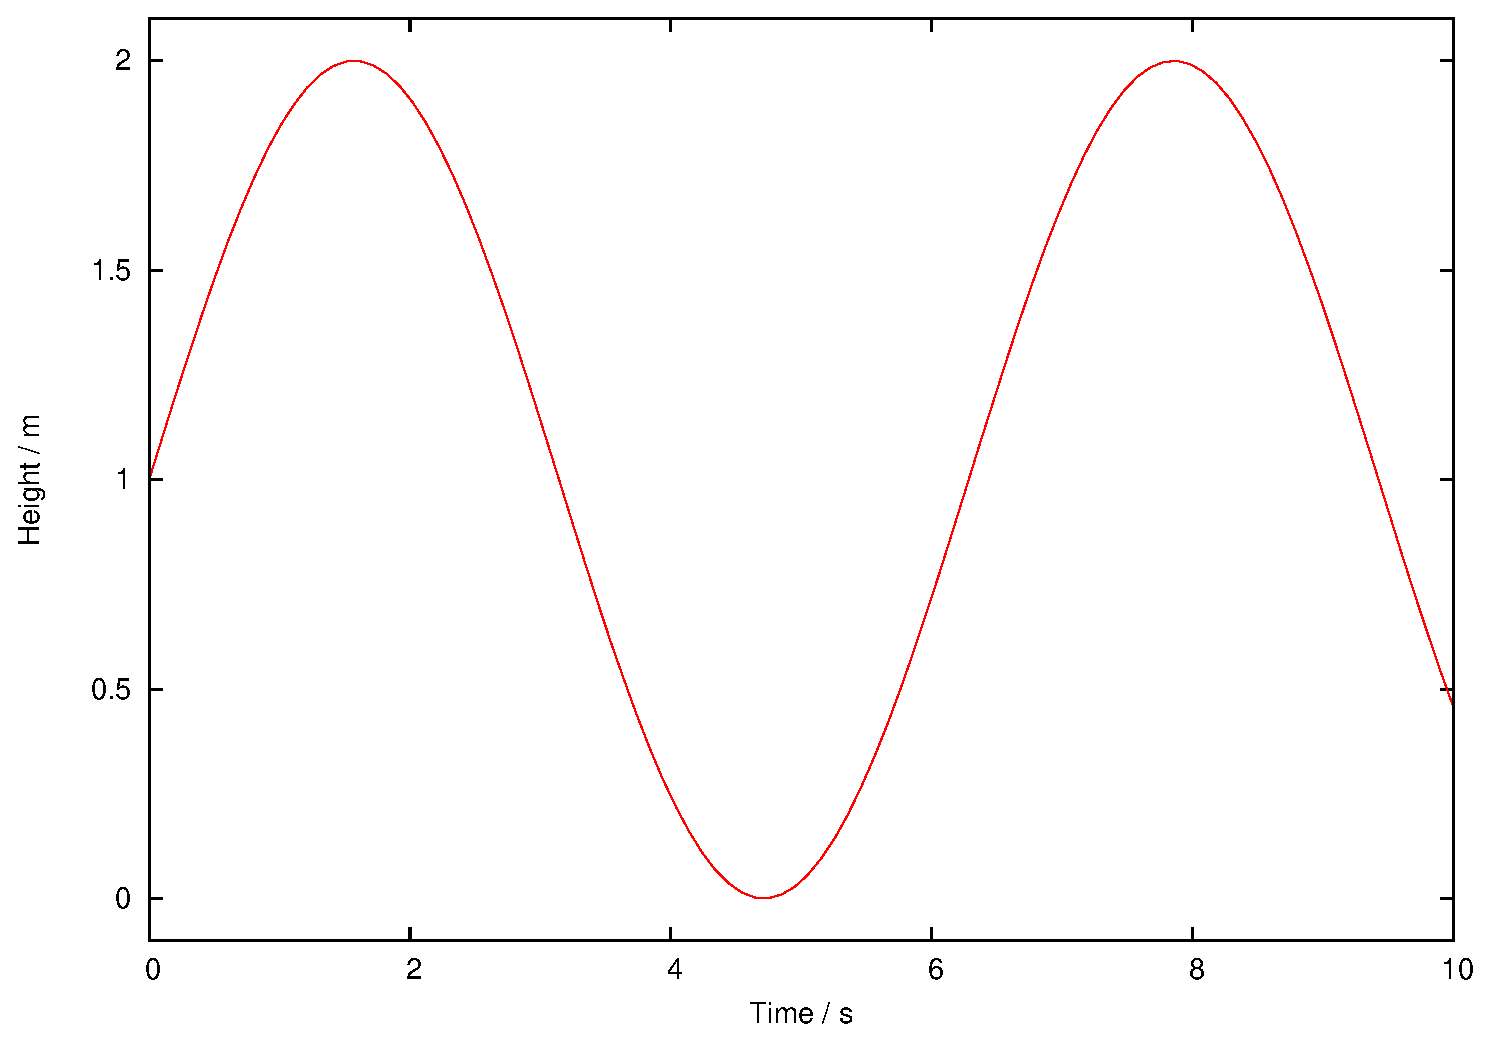
\includegraphics[width=\columnwidth]{example}
%     \caption{This is an example figure. Captions appear below each figure.
% 	Give enough detail for the reader to understand what they're looking at,
% 	but leave detailed discussion to the main body of the text.}
%     \label{fig:example_figure}
% \end{figure}

% % Example table
% \begin{table}
% 	\centering
% 	\caption{This is an example table. Captions appear above each table.
% 	Remember to define the quantities, symbols and units used.}
% 	\label{tab:example_table}
% 	\begin{tabular}{lccr} % four columns, alignment for each
% 		\hline
% 		A & B & C & D\\
% 		\hline
% 		1 & 2 & 3 & 4\\
% 		2 & 4 & 6 & 8\\
% 		3 & 5 & 7 & 9\\
% 		\hline
% 	\end{tabular}
% \end{table}


% \section{Conclusions}

% The last numbered section should briefly summarise what has been done, and describe
% the final conclusions which the authors draw from their work.

% \section*{Acknowledgements}

% The Acknowledgements section is not numbered. Here you can thank helpful
% colleagues, acknowledge funding agencies, telescopes and facilities used etc.
% Try to keep it short.

% %%%%%%%%%%%%%%%%%%%%%%%%%%%%%%%%%%%%%%%%%%%%%%%%%%
% \section*{Data Availability}

 
% The inclusion of a Data Availability Statement is a requirement for articles published in MNRAS. Data Availability Statements provide a standardised format for readers to understand the availability of data underlying the research results described in the article. The statement may refer to original data generated in the course of the study or to third-party data analysed in the article. The statement should describe and provide means of access, where possible, by linking to the data or providing the required accession numbers for the relevant databases or DOIs.




% %%%%%%%%%%%%%%%%%%%% REFERENCES %%%%%%%%%%%%%%%%%%

% % The best way to enter references is to use BibTeX:
\newpage
\bibliographystyle{mnras}
\bibliography{example} % if your bibtex file is called example.bib

% % Alternatively you could enter them by hand, like this:
% % This method is tedious and prone to error if you have lots of references
% %\begin{thebibliography}{99}
% %\bibitem[\protect\citeauthoryear{Author}{2012}]{Author2012}
% %Author A.~N., 2013, Journal of Improbable Astronomy, 1, 1
% %\bibitem[\protect\citeauthoryear{Others}{2013}]{Others2013}
% %Others S., 2012, Journal of Interesting Stuff, 17, 198
% %\end{thebibliography}

% %%%%%%%%%%%%%%%%%%%%%%%%%%%%%%%%%%%%%%%%%%%%%%%%%%

% %%%%%%%%%%%%%%%%% APPENDICES %%%%%%%%%%%%%%%%%%%%%

% \appendix

% \section{Some extra material}

% If you want to present additional material which would interrupt the flow of the main paper,
% it can be placed in an Appendix which appears after the list of references.

%%%%%%%%%%%%%%%%%%%%%%%%%%%%%%%%%%%%%%%%%%%%%%%%%%


% Don't change these lines
\bsp	% typesetting comment
\label{lastpage}
\end{document}

% End of mnras_template.tex
